% B.Tech project report: Knee Abnormality Detection Using Deep Learning
% Department of Electronics & Communication Engineering, Faculty of Technology, University of Delhi
% Format: FOT ECE B.Tech project report guidelines (A4; Times 12 pt; double spacing; margins L 3.5 cm,
% T 2.5 cm, R 1.25 cm, B 1.25 cm; captions Times italic 10 pt; tables Times 10 pt single spacing;
% chapter titles bold capitals 16 pt centred; headings bold 14 pt; sub-headings bold 12 pt).
% Compile: pdflatex (run three times so the contents, lists and cross-references settle).
\documentclass[12pt,a4paper,oneside]{report}

\usepackage[T1]{fontenc}
\usepackage[utf8]{inputenc}
\usepackage{newtxtext,newtxmath}            % Times Roman text and maths
\usepackage[british]{babel}
\usepackage[a4paper,left=3.5cm,right=1.25cm,top=2.5cm,bottom=1.25cm,includefoot,footskip=0.9cm]{geometry}
\usepackage{setspace}
\usepackage{graphicx}
\usepackage{booktabs,array,tabularx,multirow,makecell,longtable}
\usepackage{amsmath}
\usepackage{xcolor}
\usepackage{tikz}
\usetikzlibrary{positioning,arrows.meta,fit,calc,shapes.geometric,backgrounds}
\usepackage{etoolbox}
\usepackage{enumitem}
\usepackage{titlesec}
\usepackage{tocloft}
\usepackage[font={footnotesize,it},labelfont={footnotesize,it},justification=centering,singlelinecheck=false,skip=6pt]{caption}
\usepackage{float}
\usepackage{cite}
\renewcommand{\citepunct}{],\penalty\citepunctpenalty\ [}
\renewcommand{\citedash}{]--[}
\usepackage[hidelinks,bookmarksnumbered]{hyperref}
\usepackage{xurl}
\urlstyle{same}

\graphicspath{{figures/}}

% ---------------------------------------------------------------- line spacing
\doublespacing
% tables: Times 10 pt (\footnotesize in a 12 pt document), single spacing. A float resets the font size after
% environment hooks run, so every table sets \footnotesize\setstretch{1} itself; longtable is not a float.
\AtBeginEnvironment{longtable}{\footnotesize\setstretch{1}}
\setlength{\tabcolsep}{4pt}
% float pages start at the top instead of being centred vertically
\makeatletter
\setlength{\@fptop}{0pt}
\setlength{\@fpsep}{14pt}
\setlength{\@fpbot}{0pt plus 1fil}
\makeatother
\renewcommand{\floatpagefraction}{0.6}
\renewcommand{\topfraction}{0.85}
\renewcommand{\textfraction}{0.12}
\renewcommand{\arraystretch}{1.25}
% captions: figure caption at the bottom, table caption at the top, both centred, italic 10 pt
\captionsetup[table]{position=top}
\captionsetup[figure]{position=bottom}
\renewcommand{\figurename}{Figure}
\renewcommand{\tablename}{Table}
\captionsetup{labelsep=space}
\DeclareCaptionLabelFormat{dotted}{#1 #2:}
\captionsetup{labelformat=dotted}

% ---------------------------------------------------------------- headings
\titleformat{\chapter}[display]
  {\centering\bfseries\fontsize{16}{20}\selectfont}
  {CHAPTER \thechapter}{6pt}{\MakeUppercase}
\titlespacing*{\chapter}{0pt}{-12pt}{24pt}
\titleformat{\section}{\bfseries\fontsize{14}{17}\selectfont}{\thesection}{0.8em}{}
\titleformat{\subsection}{\bfseries\fontsize{12}{14.5}\selectfont}{\thesubsection}{0.8em}{}
\titleformat{\subsubsection}[runin]{\bfseries\fontsize{12}{14.5}\selectfont}{}{0pt}{}[.]
\titlespacing*{\section}{0pt}{10pt}{4pt}
\titlespacing*{\subsection}{0pt}{8pt}{2pt}
\titlespacing*{\subsubsection}{0pt}{6pt}{0.6em}
\setcounter{secnumdepth}{2}
\setcounter{tocdepth}{2}

% unnumbered front-matter and back-matter titles in the chapter-title style
\newcommand{\frontchapter}[1]{%
  \chapter*{#1}\addcontentsline{toc}{chapter}{\texorpdfstring{\textit{#1}}{#1}}}
\newcommand{\backchapter}[1]{%
  \chapter*{#1}\addcontentsline{toc}{chapter}{#1}}

% ---------------------------------------------------------------- contents and lists
\addto\captionsbritish{%
  \renewcommand{\contentsname}{CONTENTS}%
  \renewcommand{\listfigurename}{LIST OF FIGURES}%
  \renewcommand{\listtablename}{LIST OF TABLES}%
  \renewcommand{\bibname}{REFERENCES}%
  \renewcommand{\figurename}{Figure}%
  \renewcommand{\tablename}{Table}}
\renewcommand{\cftchapfont}{\bfseries}
\renewcommand{\cftchappagefont}{\bfseries}
\renewcommand{\cftchappresnum}{CHAPTER~}
\setlength{\cftchapnumwidth}{6.6em}
\renewcommand{\cftfigpresnum}{Figure~}
\renewcommand{\cfttabpresnum}{Table~}
\setlength{\cftfignumwidth}{5.4em}
\setlength{\cfttabnumwidth}{5.0em}
\setlength{\cftbeforefigskip}{2pt}
\setlength{\cftbeforetabskip}{2pt}
\setlength{\cftbeforechapskip}{6pt}
\renewcommand{\cftdotsep}{2}
\setlength{\cftbeforetoctitleskip}{-12pt}
\setlength{\cftbeforeloftitleskip}{-12pt}
\setlength{\cftbeforelottitleskip}{-12pt}
\renewcommand{\cfttoctitlefont}{\hfill\bfseries\fontsize{16}{20}\selectfont}
\renewcommand{\cftaftertoctitle}{\hfill\hfill}
\renewcommand{\cftloftitlefont}{\hfill\bfseries\fontsize{16}{20}\selectfont}
\renewcommand{\cftafterloftitle}{\hfill\hfill}
\renewcommand{\cftlottitlefont}{\hfill\bfseries\fontsize{16}{20}\selectfont}
\renewcommand{\cftafterlottitle}{\hfill\hfill}

% ---------------------------------------------------------------- lists and misc
\setlist{itemsep=0pt,topsep=2pt,parsep=0pt,partopsep=0pt}
\newcolumntype{L}[1]{>{\raggedright\arraybackslash}p{#1}}
\newcolumntype{C}[1]{>{\centering\arraybackslash}p{#1}}
\newcolumntype{Y}{>{\raggedright\arraybackslash}X}
\newcommand{\auc}{\mbox{AUC}}
\hyphenation{Conv-NeXt Efficient-Net Kaggle pre-processing}

% TikZ styles shared by the block diagrams
\tikzset{
  blk/.style={draw=black!70, rounded corners=2pt, align=center, font=\footnotesize, inner sep=3pt, minimum height=8mm, fill=white, execute at begin node={\hyphenpenalty=10000\exhyphenpenalty=10000}},
  data/.style={blk, fill=black!6},
  ours/.style={blk, fill=blue!8, draw=blue!60!black},
  pub/.style={blk, fill=orange!10, draw=orange!70!black},
  arr/.style={-{Stealth[length=2.2mm]}, thick, draw=black!75},
  lbl/.style={font=\scriptsize\itshape, text=black!75, align=center},
}

\begin{document}

% ---------------------------------------------------------------- title page (no page number)
\pagenumbering{alph}
% Title page, laid out after the department's sample sheet (title page / front page).
\begin{titlepage}
\singlespacing
\centering
{\fontsize{14}{17}\selectfont\bfseries Project Report\par}
\vspace{4pt}
{\fontsize{14}{17}\selectfont\bfseries on\par}
\vspace{12pt}
{\fontsize{14}{18}\selectfont\bfseries KNEE ABNORMALITY DETECTION USING DEEP LEARNING\par}
\vspace{18pt}
{\fontsize{12}{15}\selectfont SUBMITTED IN PARTIAL FULFILMENT OF THE REQUIREMENT FOR THE AWARD\\[3pt]
OF THE DEGREE OF\par}
\vspace{18pt}
{\fontsize{14}{17}\selectfont\bfseries BACHELOR OF TECHNOLOGY\par}
\vspace{6pt}
{\fontsize{14}{17}\selectfont (Electronics \& Communication Engineering)\par}
\vspace{24pt}

\includegraphics[height=4.2cm]{figures/du_logo.jpeg}\par
\vspace{22pt}
{\fontsize{14}{17}\selectfont Session: 2026--2027\par}
\vspace{30pt}
{\fontsize{12}{15}\selectfont
\begin{minipage}[t]{0.50\textwidth}
\raggedright
\textbf{SUBMITTED BY:}\\[6pt]
NAME(S) \& UNIVERSITY ROLL NO.(s):\\[4pt]
Nishkarsh Singhal \hfill 24294917099\\[2pt]
Anuj Chaubey \hfill 24294917055\\[2pt]
Vardhan Harsh Nigam \hfill 24294917014\\[2pt]
B.Tech (ECE), Section B
\end{minipage}\hfill
\begin{minipage}[t]{0.42\textwidth}
\raggedright
\textbf{UNDER THE GUIDANCE OF:}\\[6pt]
NAME: Dr. Varun Saxena\\[2pt]
DESIGNATION: Associate Professor,\\
Department of Electronics \&\\ Communication Engineering\\[8pt]
NAME: Dr. Sangeeta Yadav\\[2pt]
DESIGNATION: Assistant Professor,\\
Department of Computer Science \&\\ Engineering\\[2pt]
(Co-Supervisor)
\end{minipage}\par}
\vfill
{\fontsize{12}{15}\selectfont DEPARTMENT OF ELECTRONICS \& COMMUNICATION ENGINEERING\par}
\vspace{6pt}
{\fontsize{14}{17}\selectfont FACULTY OF TECHNOLOGY\par}
\vspace{4pt}
{\fontsize{14}{17}\selectfont UNIVERSITY OF DELHI\par}
\end{titlepage}


% ---------------------------------------------------------------- preliminary pages (roman numbers)
\pagenumbering{roman}
\setcounter{page}{1}
% Preliminary pages in the order required by the department's guidelines (item 4): candidate's declaration,
% abstract, acknowledgement, list of figures, list of tables, definitions/acronyms/abbreviations, contents.

% ---------------------------------------------------------------- declaration (page i)
\clearpage
\phantomsection
\addcontentsline{toc}{chapter}{\texorpdfstring{\textit{Candidate's Declaration}}{Candidate's Declaration}}
\begin{center}
{\singlespacing\bfseries\fontsize{16}{20}\selectfont FACULTY OF TECHNOLOGY\\[4pt] UNIVERSITY OF DELHI\par}
\end{center}
\vspace{10pt}
\begin{center}
{\bfseries\fontsize{12}{15}\selectfont CANDIDATE'S DECLARATION}
\end{center}
\vspace{4pt}
We hereby certify that the work which is being presented in the Project entitled ``Knee Abnormality Detection Using Deep Learning'' by ``Nishkarsh Singhal, Anuj Chaubey and Vardhan Harsh Nigam'' in partial fulfilment of requirements for the award of degree of B.Tech.\ (Electronics and Communication Engineering) submitted to the Department of Electronics and Communication Engineering at Faculty of Technology, University of Delhi, Delhi is an authentic record of our own work carried out during a period from August 2026 to November 2026. The matter presented in this project has not been submitted by us or anybody else in any other University / Institute.

Public models, code and label sets released by other participants of the RSNA Knee Abnormality Detection challenge were used where stated in the report and are acknowledged in the text and in the references.

\vspace{1.2cm}
\noindent\textbf{Signature of the Students}

\vspace{0.6cm}
{\singlespacing
\noindent\begin{tabular}{@{}p{5.0cm}p{5.0cm}p{5.0cm}@{}}
\rule{4.4cm}{0.4pt} & \rule{4.4cm}{0.4pt} & \rule{4.4cm}{0.4pt} \\
Nishkarsh Singhal & Anuj Chaubey & Vardhan Harsh Nigam \\
Roll No.\ 24294917099 & Roll No.\ 24294917055 & Roll No.\ 24294917014 \\
\end{tabular}}

\vspace{1.6cm}
{\singlespacing
\noindent\begin{tabular}{@{}>{\raggedright\arraybackslash}p{7.6cm}>{\raggedright\arraybackslash}p{7.6cm}@{}}
\rule{5.6cm}{0.4pt} & \rule{5.6cm}{0.4pt} \\
\textbf{Dr.\ Varun Saxena} & \textbf{Dr.\ Sangeeta Yadav} \\
Associate Professor (Project Supervisor) & Assistant Professor (Co-Supervisor) \\
Department of Electronics \& Communication Engineering & Department of Computer Science \& Engineering \\
Faculty of Technology, University of Delhi & Faculty of Technology, University of Delhi \\
\end{tabular}}

\begin{center}{\footnotesize\bfseries (Signature and Name of Project Guide/Guides)}\end{center}

% ---------------------------------------------------------------- abstract (page ii, not more than one page)
\frontchapter{Abstract}
{\setstretch{1.75}
This project developed a deep learning system that reads a complete knee MRI study in DICOM format and estimates the probability of twelve abnormalities, including ligament and meniscal tears, osteoarthritis, joint effusion and bone injuries. It was built on the data of the RSNA Knee Abnormality Detection challenge on Kaggle: 4,407 training studies, of which only 58 carry expert labels, while the rest have free-text reports in nine languages. We first audited the data and replaced an unreliable labelling pipeline with a language model run locally in a forced-choice mode. Its labels agreed with the expert labels at a macro AUC of 0.868, or 0.890 after averaging with two public label sets. On these labels we trained a fine-tuned 2.5D multiple-instance network with one attention head per finding, which raised the leaderboard score of our frozen-feature baseline from 0.775 to 0.927 (0.916 on the private leaderboard). In the final week we built ensembles around the strongest public models, after tracing their training data and re-running each one locally, and re-engineered one inference pipeline so that an extra model fitted within the nine-hour limit; the best entry scored 0.943 on the private leaderboard and placed the team 490th of 6,299 teams, with a bronze medal. After the competition, an experiment in which only the training labels were changed showed that the labels limited our model more than its design: labels read from the images raised its gold-set AUC from 0.891 to 0.928. We then retrained the winning team's published box-pooling pipeline. It reproduced the published single-model score (0.955 against 0.954), and training it on the mean of two published image-read label sets gave 0.958 on the private leaderboard, where the winning team scored 0.960. Last, we built a local workstation that runs the final models on a 6~GB laptop GPU, matches our Kaggle inference script to within $1.6\times10^{-4}$, and shows for each model an exact breakdown of its score over image regions.\par}

\vspace{6pt}
\noindent\textbf{Keywords:} knee MRI, deep learning, multiple-instance learning, weak supervision, report-derived labels, ConvNeXt, explainability.

% ---------------------------------------------------------------- acknowledgement (page iii)
\frontchapter{Acknowledgement}
We are grateful to our project supervisor, Dr.\ Varun Saxena, Associate Professor in the Department of Electronics and Communication Engineering, for guidance and encouragement throughout this project, and for giving us the freedom to explore the problem in our own way. We thank our co-supervisor, Dr.\ Sangeeta Yadav, Assistant Professor in the Department of Computer Science and Engineering, for advice on the machine learning side of the work and for careful questions about how we evaluated our models.

We thank the Department of Electronics and Communication Engineering, Faculty of Technology, University of Delhi, for the opportunity to take up this project. We thank the Radiological Society of North America and Kaggle for organising the RSNA Knee Abnormality Detection challenge and making its data available for research, and Kaggle for the free GPU time without which the larger models could not have been trained.

Several participants of the challenge shared their work openly, and this project depended on it. We thank the first-placed team, Team Kangaroo, for publishing their training code and labels, the seventh-placed team for publishing their label set, and the authors of the public models and label sets that we used during the competition.

We also thank our families and friends for their patience during the long hours that this project took.

\vspace{1cm}
\noindent\begin{tabular}{@{}l@{}}
Nishkarsh Singhal\\ Anuj Chaubey\\ Vardhan Harsh Nigam
\end{tabular}

% ---------------------------------------------------------------- lists
\cleardoublepage
\phantomsection
\addcontentsline{toc}{chapter}{\texorpdfstring{\textit{List of Figures}}{List of Figures}}
{\singlespacing\listoffigures}

\cleardoublepage
\phantomsection
\addcontentsline{toc}{chapter}{\texorpdfstring{\textit{List of Tables}}{List of Tables}}
{\singlespacing\listoftables}

% ---------------------------------------------------------------- definitions, acronyms and abbreviations
\frontchapter{Definitions, Acronyms and Abbreviations}
{\singlespacing\footnotesize
\begin{longtable}{@{}L{3.0cm}L{12.0cm}@{}}
\toprule
\textbf{Term} & \textbf{Meaning} \\
\midrule
\endhead
2.5D & input made of a few neighbouring slices stacked as the channels of one 2D image \\
ACL / MCL & anterior cruciate ligament / medial collateral ligament \\
Ablation & an experiment that changes one part of a system to measure that part's effect \\
AdamW & Adam optimiser with decoupled weight decay \\
AUC, ROC-AUC & area under the receiver operating characteristic curve \\
AWQ & activation-aware weight quantisation, a 4-bit format for language-model weights \\
Baker's cyst & fluid-filled (popliteal) cyst behind the knee \\
bfloat16, fp16, fp32 & 16-bit brain floating point, 16-bit and 32-bit IEEE floating point \\
CI & confidence interval (95\% unless stated otherwise) \\
CNN & convolutional neural network \\
DDP & distributed data parallel (training on several GPUs) \\
DICOM & Digital Imaging and Communications in Medicine, the file format of medical images \\
Drop-path & regularisation that randomly skips residual blocks of a network during training \\
EMA & exponential moving average of the network weights \\
FiLM & feature-wise linear modulation: scaling and shifting features according to side information \\
FS & fluid-sensitive (fat-suppressed) MRI sequence \\
Feature pyramid & network part that combines feature maps of several resolutions from coarse to fine \\
Gold-58 & the 58 training studies with expert labels for all twelve findings \\
Fold, held-out fold & one of five disjoint subsets of the report-labelled studies; a fold left out of training and used for validation. \emph{Our fold~0} (Stages 3 and 5) and \emph{the published fold~0} (box-pooling models) are different sets of 870 studies \\
Image-read labels & labels made by reading the images (here by LLM agents of other teams), as opposed to labels taken from the report \\
In-sample & measured on the same data that was used to fit or choose something, and therefore optimistic \\
KV cache & key--value cache: stored intermediate results of a language model for text it has already read \\
Late submission & a submission scored after the competition closed; it receives a score but no rank \\
Logit & score of a finding before the sigmoid function turns it into a probability \\
JSON, NDJSON & JavaScript Object Notation; newline-delimited JSON \\
LB & leaderboard (public: part of the hidden test set; private: the rest, revealed at the end) \\
LLM & large language model \\
MIL & multiple-instance learning \\
MRI & magnetic resonance imaging \\
NF4 & 4-bit NormalFloat weight quantisation \\
OA, PF OA & osteoarthritis; patellofemoral osteoarthritis \\
OAI & Osteoarthritis Initiative (public knee cohort study) \\
ROI & region of interest \\
Seed & number that fixes the random initialisation, data order and augmentation of a training run \\
Soft label & a training target between 0 and 1 instead of exactly 0 or 1 \\
Spearman correlation & correlation between the ranks of two sets of values \\
T (field strength) & tesla \\
TensorRT & NVIDIA library that compiles a trained network for faster inference \\
TTA & test-time augmentation (averaging predictions over transformed inputs) \\
vLLM & open-source serving engine for large language models \\
VRAM & memory on the graphics card \\
\midrule
\multicolumn{2}{@{}l}{\textbf{Names of label sets, runs and submissions}} \\
\midrule
P1, P2 & two report-derived label sets published by other participants during the competition \\
E0, E1, E1p, \dots & training runs of our 2.5D model (E0: frozen-feature design; E1: reference run; E1p: with the slice-position fix; E9: higher resolution) \\
F1--F3 & the three final models of Stage 3, trained on all report-labelled studies \\
A0, A1, A2, C1--C3 & box-pooling runs of Stage 5 (Table~\ref{tab:bpruns}) \\
CoAtNet, S6, s6fall, R6 & public models used in Stage 4 (Table~\ref{tab:public}) \\
A-strict, final-strict, final-max & names of our Stage 4 submissions (Table~\ref{tab:endgame}) \\
\midrule
\multicolumn{2}{@{}l}{\textbf{Notation}} \\
\midrule
$y_{ik}$ & training label of study $i$ for finding $k$, a number in $[0,1]$ \\
$\hat p_{ik}$ & predicted probability of finding $k$ in study $i$ \\
$z_k$, $\sigma(\cdot)$ & logit of finding $k$; logistic (sigmoid) function \\
$S$ & macro AUC over the twelve findings (Equation~\ref{eq:macroauc}) \\
$\mathbf t_j$, $\alpha_{k,j}$ & token of window $j$; attention weight of finding $k$ on window $j$ \\
$\phi$ & soft score of the forced-choice labeller (Equation~\ref{eq:s0}) \\
$\mu_r$, $g$ & centre slice of window $r$; slice step inside a window \\
$\mathbf f_{n,c}$, $w_{k,n,c}$ & feature of cell $c$ on slice $n$; box-pooling weight of that cell for finding $k$ \\
$s$ & attention sharpening factor applied at inference \\
$\Delta$, $R$ & paired difference in macro AUC between two models; number of bootstrap resamples \\
\multicolumn{2}{@{}l}{Indices: $i$ study, $k$ finding, $j$ window token, $n$ slice, $c$ feature cell.} \\
\bottomrule
\end{longtable}}

% ---------------------------------------------------------------- contents (after the lists, as the guidelines require)
\cleardoublepage
{\singlespacing\tableofcontents}


% ---------------------------------------------------------------- chapters (arabic numbers)
\cleardoublepage
\pagenumbering{arabic}
\setcounter{page}{1}
% ======================================================================
\chapter[INTRODUCTION \& PROJECT FORMULATION]{Introduction \& Project Formulation}
\label{ch:intro}
% ======================================================================

\section{Overview}

Magnetic resonance imaging (MRI) is widely used to examine the soft tissues of the knee, such as the ligaments, menisci and cartilage, which plain X-ray images do not show well \cite{bien2018}. A single knee study contains several image series. Each series is a stack of thin slices taken in one of three planes with one of several pulse sequences. A radiologist reads all of them and writes a free-text report that states which structures are torn, worn, swollen or bruised.

This project builds a deep learning system that reads a complete knee MRI study, exactly as it comes out of the scanner in DICOM format, and gives a probability for each of twelve abnormalities. The work was carried out on the data of the RSNA Knee Abnormality Detection challenge, a public machine learning competition hosted on Kaggle by the Radiological Society of North America (RSNA) \cite{kaggle_rsna_knee,rsna2026announce}. The competition provided a large multi-centre dataset and a test set whose labels were hidden from all teams. Because of this, the leaderboard gave an independent check of the design decisions we made.

\subsection{Clinical background}

The knee joint is formed by the femur, the tibia and the patella. Its stability depends on four main ligaments, two of which, the anterior cruciate ligament (ACL) and the medial collateral ligament (MCL), are among the findings studied here. Two C-shaped pads of fibrocartilage, the medial and lateral menisci, sit between the femur and the tibia and spread the load across the joint. The joint surfaces are covered with articular cartilage, and its gradual loss is called osteoarthritis (OA). Radiologists describe OA separately for the medial and lateral tibiofemoral compartments and for the patellofemoral (PF) compartment behind the kneecap.

Besides these structural findings, a report usually comments on the fluid inside the joint (an effusion), on thickening and inflammation of the joint lining (synovitis), on a fluid-filled Baker's cyst behind the knee, and on the bones themselves, which can show a bruise (bone contusion) or a fracture after trauma. Some of these findings are focal and visible on two or three slices, such as a meniscal tear. Others, such as an effusion, are spread over a large part of the joint. A useful system therefore has to look at the right part of the right series for each finding.

A knee MRI study is acquired in three planes. Sagittal slices are stacked from one side of the knee to the other, and each shows a front-to-back view in which the cruciate ligaments and the menisci are seen along their length. Coronal slices are stacked from front to back and show the collateral ligaments and the medial and lateral compartments side by side. Axial slices are horizontal and show the patellofemoral joint and the fluid pockets around it. Each plane is usually imaged with a fluid-sensitive, fat-suppressed sequence, in which fluid and oedema appear bright, and often also with a sequence without fat suppression that shows anatomy more clearly.

\subsection{The RSNA knee abnormality detection challenge}

The task set by the organisers is to predict, for each test study, the probability that each of the twelve findings in Table~\ref{tab:targets} is present. The study is the unit of prediction: there is one row per study in the submission file, whatever the number of series it contains.

\begin{table}[htbp]
\centering\footnotesize\setstretch{1}
\caption[The twelve findings and their gold-58 positives]{The twelve findings predicted by the system, with the competition's definitions and the number of positive studies among the 58 expert-labelled training studies}
\label{tab:targets}
\begin{tabular}{L{3.2cm}L{8.4cm}C{2.2cm}}
\toprule
Target column & Definition used by the organisers & Positives in gold-58 \\
\midrule
ACL & anterior cruciate ligament injury & 24 \\
MCL & medial collateral ligament injury & 9 \\
Medial Meniscus & tear of the medial meniscus & 26 \\
Lateral Meniscus & tear of the lateral meniscus & 23 \\
Medial OA & osteoarthritis of the medial tibiofemoral compartment & 15 \\
Lateral OA & osteoarthritis of the lateral tibiofemoral compartment & 11 \\
PF OA & patellofemoral osteoarthritis & 21 \\
Effusion & joint effusion (excess fluid in the joint) & 35 \\
Synovitis & inflammation of the joint lining & 27 \\
Baker's & Baker's (popliteal) cyst & 12 \\
Contusion & bone contusion (bone bruise) & 19 \\
Fracture & fracture & 18 \\
\bottomrule
\end{tabular}
\end{table}

\paragraph{Evaluation metric.} Submissions are scored with the macro-averaged area under the receiver operating characteristic curve (ROC-AUC) \cite{hanley1982,fawcett2006}. For a finding $k$, the AUC is the probability that a randomly chosen positive study receives a higher score than a randomly chosen negative study,
\begin{equation}
\auc_k=\frac{1}{|P_k|\,|N_k|}\sum_{i\in P_k}\sum_{j\in N_k}\Big[\mathbf{1}(\hat p_{ik}>\hat p_{jk})+\tfrac12\,\mathbf{1}(\hat p_{ik}=\hat p_{jk})\Big],
\label{eq:auc}
\end{equation}
where $P_k$ and $N_k$ are the positive and negative test studies for that finding, $\hat p_{ik}$ is the predicted probability, and $\mathbf{1}(\cdot)$ is one when its condition holds and zero otherwise. The competition score is the plain mean over the twelve findings,
\begin{equation}
S=\frac{1}{12}\sum_{k=1}^{12}\auc_k .
\label{eq:macroauc}
\end{equation}
Because the AUC depends only on the order of the scores, the metric does not reward calibrated probabilities or a good choice of threshold. It rewards ranking the positive studies above the negative ones, separately for every finding. A rare finding such as MCL injury counts exactly as much as a common one such as effusion.

\paragraph{Training data.} The training set contains 4,407 knee MRI studies with their DICOM files and one radiology report per study. Only 58 of these studies carry expert labels for all twelve findings. We call them the \emph{gold-58} set throughout this report. The other 4,349 studies have a report and nothing else. The reports are written in nine languages and were produced in routine clinical work, so they follow each hospital's habits rather than a fixed template. Reports are not available for test studies. They can be used to create training labels, but the model itself has to work from the images alone.

\paragraph{Test data and rules.} The hidden test set has about 1,300 studies. It is swapped in only when a submitted notebook is scored, so participants never see it. The competition was run as a \emph{code competition}: a submission is a Kaggle notebook that must read the raw test DICOMs and write the predictions within nine hours of run time, with internet access switched off. Freely and publicly available external data and pretrained models were allowed. Each team could make five submissions per day and select two final submissions for the private leaderboard. The data licence allows research use but forbids passing the data on to anyone outside the competition \cite{kaggle_rsna_knee}. Apart from one workstation screenshot of a public example study, this report therefore shows statistics and diagrams rather than MRI images from the dataset. These rules (nine hours, no internet, five submissions a day, no redistribution) are referred to in later chapters without being repeated.

\subsection{Characteristics of the dataset}

Before any modelling we audited the full dataset: every series, every DICOM header and every report. The main numbers are collected in Table~\ref{tab:dataset} and Figure~\ref{fig:dataset}.

\begin{table}[htbp]
\centering\footnotesize\setstretch{1}
\caption{Summary of the training data, measured over all files in our audit}
\label{tab:dataset}
\begin{tabular}{L{7.2cm}L{6.8cm}}
\toprule
Quantity & Value \\
\midrule
Studies (gold-labelled / report only) & 4,407 (58 / 4,349) \\
Series / DICOM files / size on disk & 24,371 / 819,078 / 569~GB (uncompressed) \\
Series per study & median 5 (range 3--14) \\
Slices per study & median 162 (range 67--632) \\
Studies with all three planes & 4,407 (100\%) \\
Fluid-sensitive series missing & sagittal 257, coronal 159, axial 0 studies \\
Laterality tag present in the DICOM header & 2,204 studies (50\%) \\
Report languages & 9 (English, Spanish, Turkish, Croatian, Greek, German, Bulgarian, Dutch, French) \\
Patient identifiers & pseudonymised per study (4,407 unique) \\
Pixel-identical duplicate studies & 1 pair, with two conflicting reports \\
\bottomrule
\end{tabular}
\end{table}

\begin{figure}[htbp]
\centering\setstretch{1}
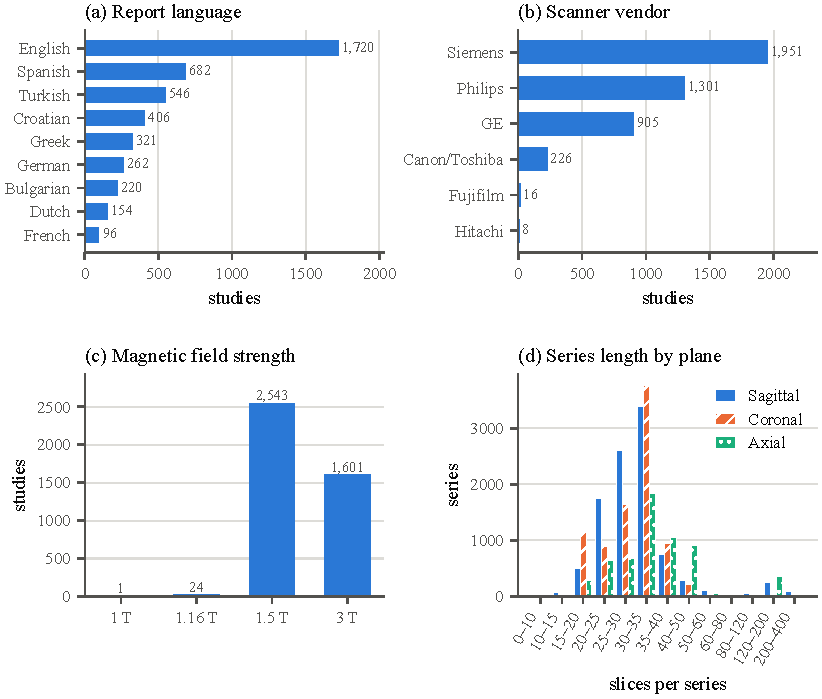
\includegraphics[width=\textwidth]{fig_dataset.pdf}
\caption[Composition of the training studies]{Composition of the 4,407 training studies: (a) report language, (b) scanner vendor, (c) field strength where the header records it, and (d) the number of slices per series in each plane}
\label{fig:dataset}
\end{figure}

Several of these properties shaped the project from the start. Language, hospital and scanner vendor are tied together: all Bulgarian studies come from Philips scanners, and all German, Greek and Dutch studies from Siemens scanners. Raw intensity values differ by a factor of about 25 between vendors, so no fixed intensity window can be used. Almost every study has more than one sagittal series, and some three-dimensional acquisitions contain up to 320 slices, while a typical two-dimensional series has about 30 slices that are 3--4~mm apart. A 512-pixel image may cover anything from 120 to 200~mm, so the physical size of a pixel varies between studies.

The orientation of the images also matters. In the coronal and axial planes, a right knee shows its lateral side on the left of the image and a left knee shows it on the right. A model that is not told which knee it sees has to learn every medial and lateral finding twice. The DICOM laterality tag is present for only about half of the studies, but we found that the side can be recovered for every series from the patient coordinates stored in the header, with 97.8\% agreement with the tag where both exist.

The gold-58 set is also unusual. Every gold study has at least one positive finding, with 4.1 positives per study on average, so the set contains no normal knees. Participants in the competition reported that these labels came from radiologists reading the images rather than the report. We could not confirm this from an official source. Our own measurements in Chapter~3 agree with it, because the reports leave out about half of the synovitis that the gold labels mark as present.

\subsection{Existing systems}

\paragraph{Deep learning on knee MRI.} Deep learning for knee and other joint MRI has been surveyed in a recent scoping review \cite{fritz2022review}. The best known earlier system is MRNet \cite{bien2018}. It was trained on 1,370 knee examinations from Stanford University Medical Center and predicts three labels: any abnormality, ACL tear and meniscal tear. MRNet runs a two-dimensional convolutional network (AlexNet) on every slice of a series, takes the maximum of the slice features, and combines the three planes with logistic regression. On its own hospital's data it reached an AUC of 0.965 for ACL tears, but on an external dataset of 917 examinations from a hospital in Croatia the same model scored 0.824 before it was retrained \cite{bien2018,stajduhar2017}. A model can learn the habits of one site, and this matters here because the competition data comes from many sites and scanners.

Other public knee datasets serve different purposes. The KneeMRI dataset of {\v S}tajduhar \emph{et al.} \cite{stajduhar2017} grades ACL injury on sagittal volumes from one Croatian hospital. fastMRI \cite{zbontar2018fastmri} was built for image reconstruction from raw scanner data, and fastMRI+ \cite{zhao2022fastmriplus} later added pathology annotations to part of it. The Osteoarthritis Initiative (OAI) \cite{nevitt_oai} is a long-term cohort study with MRI and expert grading of knee osteoarthritis. None of these datasets covers the twelve findings of this task with one consistent set of labels.

\paragraph{Learning from study-level labels.} A study-level label says that a finding is present somewhere in the study but does not say on which slice. Multiple-instance learning (MIL) treats the study as a bag of instances (slices or groups of slices) with one label for the whole bag. Attention-based MIL \cite{ilse2018} learns a weight for each instance and pools the instance features with these weights. The weights are learned from the bag label alone and often point to the instances that carry the finding. This idea is the core of the image model developed in this project.

\paragraph{Image encoders.} A convolutional neural network (CNN) applies small learned two-dimensional filters to an image, much like a bank of FIR filters applied along two axes, and stacks many such layers with non-linear functions between them so that later layers respond to larger and more complex patterns. Training such a network from scratch needs far more labelled images than medical datasets usually have. The usual practice is therefore to start from a network that was \emph{pretrained} on a large collection of natural photographs such as ImageNet \cite{deng2009imagenet}, and then \emph{fine-tune} it, that is, continue training all its weights on the medical task. EfficientNet \cite{tan2019effnet,tan2021effnetv2} and ConvNeXt \cite{liu2022convnext} are two widely used families, and CoAtNet \cite{dai2021coatnet} mixes convolution with attention. Self-supervised encoders such as DINOv2 \cite{oquab2024dinov2} produce general features that can be used without training the encoder at all. We tried frozen encoders first and fine-tuned encoders later; Chapter~3 shows why the second approach was necessary.

\paragraph{Labels from radiology reports.} When images have no labels but have reports, the reports can be turned into labels. For chest X-rays, the CheXpert labeller \cite{irvin2019chexpert} used hand-written rules with explicit uncertainty classes, and CheXbert \cite{smit2020chexbert} replaced the rules with a trained language model. VisualCheXbert \cite{jain2021visualchexbert} then showed that labels read from reports disagree substantially with labels read from the images by radiologists, and that a report labeller trained to match image-based labels agrees better with radiologists who read the images. In this report we call labels of the second kind \emph{image-read labels}. Large language models (LLMs) such as the Qwen family \cite{qwen2025qwen25,yang2025qwen3} can read reports in many languages without task-specific training, which makes them attractive for multilingual data like ours.

\paragraph{Approaches in the competition.} Many teams shared notebooks and label sets during the competition. The strongest public notebooks used two-dimensional encoders on stacks of three neighbouring slices (a ``2.5D'' input), pooled over slices and series with attention, and trained on labels extracted from the reports with LLMs. The highest public scores also relied on models trained with extra knee MRI data from the OAI. After the competition the top teams published their methods, and the first- and seventh-placed teams released their label sets and, in the first case, their code \cite{tascj_boxpool,songqizhou_llmlabels}; Section~\ref{sec:impl-post} describes what we took from them.

\paragraph{Gap addressed by this project.} Existing published systems either predict a few findings, depend on thousands of expert labels, or were developed on a single site. The competition data offers the opposite situation: many findings, many sites and languages, and almost no expert labels. The project therefore had to solve two problems together, the labelling problem and the image modelling problem, and had to evaluate both without a large, trusted labelled set.

\subsection{Problem statement}

Given a knee MRI study as a folder of DICOM files, estimate the probability of each of the twelve findings in Table~\ref{tab:targets}, using a model trained on 4,407 studies of which only 58 have expert labels and the rest have free-text reports in nine languages. The system must run offline on a single Kaggle GPU within nine hours for about 1,300 studies, must not use report text at prediction time, and must be evaluated in a way that does not overstate its accuracy.

\section{User Requirement Analysis}

The system has three kinds of users, and each brings its own requirements.

The first ``user'' is the competition's scoring service. It runs our notebook on the hidden test set and expects a correctly formatted file. Its requirements are strict and fully specified: one row per test study, twelve probability columns, no missing values, a run time below nine hours, and no internet access. The test DICOMs may also be compressed with JPEG-Lossless or JPEG~2000, which the local copy of the data never was, so the system must decode both.

The second group is the project team. We needed to run experiments on one laptop with a 6~GB graphics card and on Kaggle's free GPUs, compare ideas fairly, and repeat any result later. For us the important requirements were reproducibility, honest evaluation and the ability to restart long jobs after interruptions.

The third group is the audience of the final demonstration: faculty members, radiology researchers and fellow students who want to see what the model does with a study and why. They need a simple way to load a study, to see the findings with their probabilities, and to see which part of the image drove each prediction. The system must not suggest that it is fit for clinical use.

Table~\ref{tab:requirements} lists the requirements that followed from this analysis, with the section that describes how each was handled.

\begin{table}[htbp]
\centering\footnotesize\setstretch{1}
\caption{Functional (F) and non-functional (N) requirements of the system}
\label{tab:requirements}
\begin{tabularx}{\textwidth}{l Y L{2.4cm}}
\toprule
ID & Requirement & Met in \\
\midrule
F1 & Read a study as raw DICOM files, including JPEG-Lossless and JPEG~2000 compressed files, and order slices by their position in space & \S\ref{sec:impl-mil}, \S\ref{sec:testing} \\
F2 & Produce twelve probabilities per study in the competition's submission format & \S\ref{sec:impl-mil}, \S\ref{sec:impl-post} \\
F3 & Handle missing or unreadable series without silently inventing image data & \S\ref{sec:impl-mil}, \S\ref{sec:testing} \\
F4 & Turn multilingual reports into training labels for all 4,349 unlabelled studies & \S\ref{sec:impl-audit} \\
F5 & Show the predictions and the image evidence behind them for a single study & \S\ref{sec:impl-demo} \\
N1 & Run offline on one Kaggle T4 GPU within nine hours for about 1,300 studies & \S\ref{sec:impl-mil}, \S\ref{sec:impl-post} \\
N2 & Train and run on a laptop GPU with 6~GB of memory & \S\ref{sec:impl-mil}, \S\ref{sec:impl-demo} \\
N3 & Keep competition data on our machines; no report text sent to hosted services & \S\ref{sec:impl-audit}, \S\ref{sec:impl-demo} \\
N4 & Do not select our own models on the 58 gold studies; report uncertainty with confidence intervals (not followed for the last-day blends of Stage~4) & \S\ref{sec:method-eval}, \S\ref{sec:impl-endgame} \\
N5 & Make every reported number traceable to a script, a log or a leaderboard entry & \S\ref{sec:testing}, Appendix \\
\bottomrule
\end{tabularx}
\end{table}

\section{Feasibility Study}

\paragraph{Technical feasibility.} The full training data takes 569~GB uncompressed, and one study contains about 160 slices. A frozen-feature model can be trained on any machine once the features are cached, but a model that fine-tunes its image encoder must decode and process images on every training step. We had a laptop with an Intel Core i5-13420H processor, 32~GB of memory and an NVIDIA RTX~4050 Laptop GPU with 6~GB of memory. A pilot run showed that a ConvNeXt-Tiny encoder on 224-pixel inputs, with three series and eight slice windows per study, needs 3.8~GB of GPU memory and about seven minutes per epoch on this laptop, which made local training possible. Kaggle provides two NVIDIA T4 GPUs with 15~GB each for 30 hours a week per account, which was enough for larger models later in the project. Local inference of our own model took about 1.9~s per study, or about 42 minutes for 1,300 studies, well within the nine-hour limit.

\paragraph{Economic feasibility.} All software used in the project is open source, and all the compute came from the team's own laptop and the free weekly Kaggle GPU quota of our accounts. We also asked for a small GPU quota on a commercial cloud as a backup, but the request was declined and no cloud resources were used. The project therefore had no direct cost.

\paragraph{Operational feasibility.} The competition's own submission system served as the deployment target: a notebook with attached private datasets for the model weights and the Python packages that are not in Kaggle's image. The local demonstration runs on the same laptop with a local web server and needs no network connection.

\paragraph{Legal and ethical feasibility.} The data licence permits research use but not redistribution. After the data audit, derived files (labels, caches, predictions) were excluded from version control and the code repository was made private; model weights were uploaded to Kaggle only as private datasets. Sending reports to a hosted LLM service would have meant giving competition data to a third party, so the labelling pipeline was designed to run on our own GPU. External data was used only when, in our reading, it was public and accessible to every participant on equal terms, which is the general test the organisers set out in the competition forum. The system is a research prototype trained on labels that are themselves estimates; it is not a medical device and is not meant for diagnosis.

\paragraph{Schedule feasibility.} The competition had a fixed final deadline, and the post-competition work had a fixed presentation date. Long jobs were therefore planned around the hardware: one GPU job at a time on the laptop, at most two GPU sessions at a time on a Kaggle account, and a queue system that restarted interrupted runs. The feasibility findings are summarised in Table~\ref{tab:feasibility}.

\begin{table}[htbp]
\centering\footnotesize\setstretch{1}
\caption{Summary of the feasibility study}
\label{tab:feasibility}
\begin{tabularx}{\textwidth}{L{2.9cm} Y L{2.3cm}}
\toprule
Aspect & Finding & Verdict \\
\midrule
Technical & 6~GB laptop GPU sufficient for a 224-pixel ConvNeXt-T 2.5D model (3.8~GB peak); Kaggle 2$\times$T4 for larger runs; inference about 1.9~s per study & feasible \\
Economic & open-source software, own laptop, free Kaggle quota; cloud quota request declined, nothing spent & feasible at zero cost \\
Operational & Kaggle notebook as the deployment target; local web server for the demonstration & feasible \\
Legal / ethical & research licence, no redistribution, no hosted LLM for reports, external data only if freely public; not for clinical use & feasible with the stated precautions \\
Schedule & fixed deadlines, long GPU jobs; queued and restartable runs & feasible with planning \\
\bottomrule
\end{tabularx}
\end{table}

\section{Objectives of the Project}
\label{sec:objectives}

The project had the following objectives. The sections that describe the work on each are given in brackets.

\begin{enumerate}[label=\textbf{O\arabic*.}, leftmargin=2.6em]
\item Audit the competition data and its labels, and record every property that could bias training or evaluation (\S\ref{sec:impl-audit}).
\item Build a labelling pipeline that turns the multilingual reports of all 4,349 unlabelled studies into soft training labels, running entirely on local hardware (\S\ref{sec:impl-audit}).
\item Design, train and submit our own image model, a fine-tuned 2.5D multiple-instance network with one attention head per finding (\S\ref{sec:impl-mil}).
\item Set up an evaluation protocol that does not select models on the 58 gold studies, and attach confidence intervals to every comparison (\S\ref{sec:method-eval}, \S\ref{sec:testing}).
\item Produce competition submissions that run offline within the nine-hour limit and improve the leaderboard score as far as the rules and our resources allowed (\S\ref{sec:impl-endgame}).
\item After the competition, find the main bottleneck of our approach with controlled experiments and build an improved model whose score can be compared with the winning solutions (\S\ref{sec:impl-post}).
\item Build a local workstation that runs the final models on a laptop GPU and shows the evidence behind every prediction exactly as the model computes it (\S\ref{sec:impl-demo}).
\end{enumerate}

% ======================================================================
\chapter[PROJECT DESIGN]{Project Design}
\label{ch:design}
% ======================================================================

\section{Project Perspective}

The system has two halves that share the same image-processing code (Figure~\ref{fig:context}). The training half turns the 4,349 report-only studies into labelled examples and fits the image models. The inference half takes a new study as raw DICOM files and returns twelve probabilities. It runs in two places: inside a Kaggle notebook, where it reads the hidden test set and writes the submission file, and inside a local workstation, where it reads one study at a time and also shows the evidence for each finding.

A third part sits beside both halves: the evaluation layer. It holds the 58 gold studies, the held-out folds and the leaderboard scores, and it decides which changes are kept. Keeping evaluation separate from training was a deliberate design choice, because the early versions of the project had mixed the two (Section~\ref{sec:impl-audit}).

\begin{figure}[htbp]
\centering\setstretch{1}
\begin{tikzpicture}[node distance=5mm and 6mm]
\node[data, text width=30mm] (rep) {Radiology reports\\(9 languages, training only)};
\node[ours, right=of rep, text width=28mm] (lab) {Label generation\\(local LLM, rules,\\public label sets)};
\node[data, right=of lab, text width=22mm] (soft) {Soft labels\\$y\in[0,1]^{12}$};
\node[data, below=10mm of rep, text width=30mm] (dcm) {Training studies\\(DICOM, 4,407)};
\node[ours, right=of dcm, text width=28mm] (pre) {Study index and\\preprocessing};
\node[ours, right=of pre, text width=22mm] (train) {Model training\\(laptop, Kaggle)};
\node[data, right=of train, text width=16mm] (w) {Model\\weights};
\draw[arr] (rep) -- (lab); \draw[arr] (lab) -- (soft);
\draw[arr] (dcm) -- (pre); \draw[arr] (pre) -- (train); \draw[arr] (train) -- (w);
\draw[arr] (soft) -- (train);
\node[data, below=22mm of dcm, text width=30mm] (test) {New study (DICOM)};
\node[ours, right=of test, text width=28mm] (pre2) {Same preprocessing};
\node[ours, right=of pre2, text width=22mm] (inf) {Inference\\(ensemble)};
\node[data, right=of inf, yshift=6mm, text width=24mm] (sub) {submission.csv};
\node[data, right=of inf, yshift=-6mm, text width=24mm] (ws) {Workstation view};
\draw[arr] (test) -- (pre2); \draw[arr] (pre2) -- (inf); \draw[arr] (inf.east) -- (sub.west); \draw[arr] (inf.east) -- (ws.west);
\draw[arr] (w.south) |- ($(inf.north)+(0,5mm)$) -- (inf.north);
\begin{scope}[on background layer]
\node[draw=black!40, dashed, rounded corners, fit=(rep)(lab)(soft)(dcm)(pre)(train)(w), inner sep=2.5mm] (th) {};
\node[draw=black!40, dashed, rounded corners, fit=(test)(pre2)(inf)(sub)(ws), inner sep=2.5mm] (ih) {};
\end{scope}
\node[lbl, anchor=south west] at (th.north west) {training half};
\node[lbl, anchor=north west] at (ih.south west) {inference half};
\node[blk, fill=black!3, dashed, below=9mm of ih.south, minimum width=120mm] (eval) {Evaluation layer: gold-58 (sealed), held-out folds, public and private leaderboard};
\end{tikzpicture}
\caption[System context]{System context: the training half produces labels and weights; the inference half runs the same preprocessing on new studies, both on Kaggle and in the local workstation}
\label{fig:context}
\end{figure}

\section{Project Functions}

The system performs seven functions. Each one corresponds to a group of scripts in the code repository.

\begin{enumerate}[label=\arabic*., leftmargin=1.6em]
\item \textbf{Data audit and study indexing.} Read every DICOM header, group series into studies, assign each series to a plane and sequence slot, recover the knee side, and record problems such as truncated files or duplicate studies.
\item \textbf{Label generation.} Turn each report into twelve soft labels between 0 and 1, and combine several label sources into one training target.
\item \textbf{Preprocessing.} Decode the selected series, order the slices along the scanner's slice direction, normalise intensities, mirror right knees, and cut the stacks into the inputs the model expects.
\item \textbf{Training.} Fit the image models on the labelled studies with fixed recipes, save restartable checkpoints, and log held-out results for every epoch.
\item \textbf{Evaluation.} Score predictions against gold-58, held-out folds and label sets that were not used for training, with paired bootstrap confidence intervals.
\item \textbf{Inference and submission.} Package the models and their dependencies for an offline Kaggle notebook, predict the hidden test set within the time limit, and write the submission file.
\item \textbf{Visualisation.} Load a single study in a browser, run the models on the local GPU, and show the findings with the evidence behind each one.
\end{enumerate}

\section{User Characteristics}

The users of the system, described in Section~1.2, differ in what they know and what they need from it. The competition's scoring service is fully automatic and has no tolerance for format errors. The project team are engineering students with working knowledge of Python, PyTorch and machine learning but no clinical training; they use the command-line tools and notebooks directly. The demonstration audience, which includes faculty members and radiology researchers, is expected to understand the clinical findings but not the code. For them the workstation has to explain itself. It names each processing step as it runs and labels every overlay, and it states in plain words that it is a research prototype and not a diagnostic tool.

\section{Constraints}

The design had to respect the following constraints.

\begin{itemize}[leftmargin=1.4em]
\item \textbf{Labels.} Only 58 studies carry expert labels. Training must rely on labels derived from reports, which are noisy and, for some findings, systematically different from what an image reader would say.
\item \textbf{Evaluation.} With 58 gold studies, a single study can move a finding's AUC by about 0.01, and two training runs that differed only in the random seed (the number that fixes the random initialisation and data order) differed by 0.013 in gold macro AUC. Small improvements cannot be confirmed on gold-58, and choosing models by their gold score would fit them to these 58 studies.
\item \textbf{Hardware.} The laptop GPU has 6~GB of memory, shared with the display under Windows. Exceeding it silently moves memory to system RAM and slows training by a factor of 10 to 50. Long runs also made the GPU throttle its clock because of heat.
\item \textbf{Competition rules.} The limits of Section~1.1.2 apply: nine hours of run time without internet, five submissions a day and two final picks. A hidden-test run takes from under one hour to more than eight hours, and its log is not visible to the team. Kaggle's software image used Python 3.13, so every compiled package we added had to be shipped as a matching installation file, and its T4 GPUs do not support bfloat16 arithmetic.
\item \textbf{Data rules.} No redistribution of competition data, no report text sent to hosted services, and external data only if it is freely and equally available to all participants.
\item \textbf{Test-time inputs.} Reports and labels are absent at test time, so nothing derived from a report can be a model input.
\item \textbf{DICOM variation.} Compressed transfer syntaxes in the test set, missing fluid-sensitive series in some studies, very long three-dimensional series, and a laterality tag that is missing for about half of the studies.
\end{itemize}

\section{Methodology}
\label{sec:methodology}

\subsection{Development approach}

We worked in stages. Each stage ended with a measured result, and the next stage was chosen by looking at what limited that result. Figure~\ref{fig:stages} shows the six stages and the main number reached in each, and Chapter~3 describes them in order. For most of the project we followed two working rules. Before a change was tested we wrote down the rule that would decide whether it was kept, so that a lucky result could not be read as an improvement afterwards. We also recorded every decision, including the rejected ones, in a decision log together with its evidence. The main exception to the first rule, on the last day of the competition, is described in Section~\ref{sec:impl-endgame}.

\begin{figure}[htbp]
\centering\setstretch{1}
\begin{tikzpicture}[stage/.style={blk, text width=36mm, minimum height=19mm, fill=white}, node distance=5mm and 6mm]
\node[stage, fill=black!5] (s1) {\textbf{Stage 1}\\first LLM labels,\\frozen-feature models\\[2pt]\emph{public LB 0.775}};
\node[stage, fill=blue!7, right=of s1] (s2) {\textbf{Stage 2}\\data and label audit,\\new local labeller\\[2pt]\emph{label AUC 0.868 / 0.890}};
\node[stage, fill=blue!7, right=of s2] (s3) {\textbf{Stage 3}\\fine-tuned 2.5D\\MIL network\\[2pt]\emph{private LB 0.916}};
\node[stage, fill=orange!10, below=of s3] (s4) {\textbf{Stage 4}\\ensembles built around\\public models\\[2pt]\emph{private LB 0.943}};
\node[stage, fill=blue!7, left=of s4] (s5) {\textbf{Stage 5}\\label diagnosis, published\\box pooling, fused labels\\[2pt]\emph{private LB 0.958}};
\node[stage, fill=blue!7, left=of s5] (s6) {\textbf{Stage 6}\\local workstation\\with exact evidence\\[2pt]\emph{max.\ deviation $1.6\times10^{-4}$}};
\draw[arr] (s1) -- (s2); \draw[arr] (s2) -- (s3); \draw[arr] (s3) -- (s4); \draw[arr] (s4) -- (s5); \draw[arr] (s5) -- (s6);
\end{tikzpicture}
\caption[Development stages of the project]{Development stages of the project and the main result of each stage (LB: leaderboard; the Stage~2 figures are the gold-58 AUC of our labeller alone and of the three-source training labels)}
\label{fig:stages}
\end{figure}

\subsection{Evaluation methodology}
\label{sec:method-eval}

Three references were used to judge models, because none of them is good enough alone.

\paragraph{Gold-58.} The 58 expert-labelled studies were never used for training. For our own model in Stage~3, their predictions were saved in a sealed file during training and scored once, after the model choice had been fixed; the scoring script wrote a lock file before computing any metric and refused to run a second time. In Stage~4 the public models and blends were compared on gold-58, and the last-day blend weights were fitted to it (Section~\ref{sec:impl-endgame}). In Stage~5 the gold score was logged after every epoch, but the last epoch was always used. Gold-58 is the only reference that is close to the test labels in kind, but it is small and enriched.

\paragraph{Held-out folds.} For our own model the 4,349 report-only studies were split into five \emph{folds} (disjoint subsets) at study level, stratified by report language and by the number of positive findings. Patient-level grouping was impossible because patient identifiers are unique per study; the one pixel-identical duplicate pair was kept in a single fold. Fold~0 of this split (870 studies), which we call \emph{our fold~0}, was held out of training and served as the validation set. Its labels are report-derived, so in Stage~3 the held-out score measured agreement with report labels. In Stage~5 the same studies were also scored against an image-read label set that had not been used to train the model being scored. The box-pooling models of Stage~5 used the five-fold split of the published code instead. Its fold~0, which we call \emph{the published fold~0}, also has 870 studies but shares only 180 of them with ours, so the results of Chapter~3 state which split they use.

\paragraph{Leaderboard.} The public and private leaderboards score the hidden test set. They are the final judge, but a team sees only three decimals, has five submissions a day, and learns the private score only after the competition.

\paragraph{Paired bootstrap.} When two models are compared on the same studies, we resample the studies with replacement $R=2000$ times and compute the difference in macro AUC on each resample,
\begin{equation}
\Delta^{(r)} = S\big(\hat p^{\,\text{new}}_{I_r}, y_{I_r}\big) - S\big(\hat p^{\,\text{ref}}_{I_r}, y_{I_r}\big), \qquad r = 1,\dots,R,
\label{eq:bootstrap}
\end{equation}
where $I_r$ is the $r$-th resample of study indices and $S$ is the macro AUC of Equation~\eqref{eq:macroauc}. The 2.5th and 97.5th percentiles of $\Delta^{(r)}$ give a 95\% confidence interval \cite{efron1993}. Because both models are scored on the same resample, the study-to-study variation cancels and the interval is much narrower than the interval of either score alone. A change was adopted only if it passed the rule written down before the run, typically a positive point estimate with a lower confidence bound at or above zero on the held-out data.

\subsection{Design of the label generation}
\label{sec:design-labels}

The first labeller of the project asked an LLM to write a JSON object with twelve probabilities and parsed the answer with regular expressions. When parsing failed, the script wrote 0.5 for every finding without any flag, and long reports were cut to 1,200 characters. The redesigned labeller avoids free-text output altogether (Figure~\ref{fig:labeller}). The full report is placed in a prompt that defines the twelve findings and five answer letters: \textbf{A} present, \textbf{B} possible, \textbf{C} not mentioned, \textbf{D} absent and \textbf{E} prior only (a finding mentioned as history, for example a repaired ligament). The answer layout is fixed in advance (``ACL injury: \_'', ``MCL injury: \_'', and so on), and at each blank the model's next-token distribution over the five letters is read directly. The most likely letter is then written into the blank before the next item, exactly as greedy decoding would do. Nothing is parsed, so there is no failure fallback, and the probability mass on the five letters is stored as a check that the model followed the format.

\begin{figure}[htbp]
\centering\setstretch{1}
\begin{tikzpicture}[node distance=4mm and 6mm]
\node[data] (r) {Report text};
\node[ours, right=of r] (n) {Unicode\\normalisation};
\node[ours, right=of n, text width=38mm] (p) {Prompt: 12 findings,\\letters A--E,\\fixed answer layout};
\node[ours, right=of p] (q) {Qwen3-4B\\(4-bit, local GPU)};
\node[ours, below=9mm of q] (l) {letter probabilities\\$p_A,\dots,p_E$ per item};
\node[ours, left=of l] (s) {score $\phi$\\(Eq.~\ref{eq:s0}),\\two item orders};
\node[pub, left=of s] (pubL) {public label\\sets P1 and P2};
\node[data, left=of pubL] (y) {teacher label\\(mean of three)};
\draw[arr] (r) -- (n); \draw[arr] (n) -- (p); \draw[arr] (p) -- (q); \draw[arr] (q) -- (l); \draw[arr] (l) -- (s);
\draw[arr] (s) -- (pubL); \draw[arr] (pubL) -- (y);
\end{tikzpicture}
\caption[Forced-choice labelling pipeline]{Forced-choice labelling: the model never writes free text; its letter probabilities at fixed answer positions become a soft score, which is averaged with two public label sets}
\label{fig:labeller}
\end{figure}

The five probabilities are turned into one score with weights fixed before any gold evaluation,
\begin{equation}
\phi = p_A + 0.5\,p_B + 0.25\,p_E ,
\label{eq:s0}
\end{equation}
so that a definite statement counts fully, a possible finding counts half, and a historical finding counts a quarter. The model answers the items in order and can be influenced by its earlier answers, so the labeller was run twice, once with the twelve items in the given order and once reversed, and the two scores were averaged. The final training target for study $i$ and finding $k$ is the plain mean of three sources,
\begin{equation}
y_{ik} = \tfrac13\big(\bar\phi_{ik} + y^{\text{P1}}_{ik} + y^{\text{P2}}_{ik}\big),
\label{eq:teacher}
\end{equation}
where $\bar\phi$ is the order-averaged LLM score and $y^{\text{P1}}$, $y^{\text{P2}}$ are two report-derived label sets that other participants had published on Kaggle. Their files carry no record of who made them or how, and six of the 58 gold rows in P1 are identical to the gold labels, so the gold agreement of any mixture that contains P1 may be slightly optimistic. Findings that a report does not mention keep their low score; they are not masked out.

\subsection{Design of the 2.5D image model}
\label{sec:design-mil}

The image model of Stage~3 is a multiple-instance network that reads three series per study (Figure~\ref{fig:mil}).

\paragraph{Series selection.} Each study has six slots, one for each combination of plane (sagittal, coronal, axial) and sequence (fluid-sensitive or not). The model uses the three fluid-sensitive slots. If a plane has no fluid-sensitive series, the non-fluid-sensitive series of that plane is used instead, and a plane with no series at all is masked. When a slot has several candidates, the series with the most slices is chosen.

\paragraph{Slice order and intensity.} Slices are sorted by their position along the slice normal. With the row and column direction cosines $\mathbf r$ and $\mathbf c$ from the ImageOrientationPatient tag and the slice origin $\mathbf o_i$ from ImagePositionPatient,
\begin{equation}
d_i = (\mathbf r \times \mathbf c)\cdot \mathbf o_i ,
\label{eq:sliceorder}
\end{equation}
and the slices are placed in increasing order of $d_i$. Intensities are mapped to 8 bits with the series' own 1st and 99th percentiles $q_{1}$ and $q_{99}$,
\begin{equation}
u = 255\cdot\min\!\Big(1,\max\!\Big(0,\frac{v-q_{1}}{q_{99}-q_{1}}\Big)\Big),
\label{eq:norm}
\end{equation}
which removes the factor of 25 between vendors while keeping relative brightness across the slices of one series. Each slice is resized to $224\times224$ pixels.

\paragraph{Laterality.} The knee side is read from the DICOM laterality tag when it is present. Otherwise it is taken from the sign of the patient $x$ coordinate of the coronal and axial volumes, using only series that lie at least 20~mm from the midline. For right knees the coronal and axial images are mirrored left to right, and the order of the sagittal slices is reversed, so that in every study the first sagittal slice is on the lateral side.

\paragraph{2.5D windows.} A series with $T$ slices is covered by $K=8$ windows whose centre slices $\mu_r$ are spread over 4--96\% of the stack,
\begin{equation}
\mu_r = \operatorname{round}\!\Big(0.04(T-1) + r\,\frac{0.92\,(T-1)}{K-1}\Big), \qquad r = 0,\dots,K-1 .
\label{eq:centres}
\end{equation}
Each window stacks three slices $\{\mu_r-g,\;\mu_r,\;\mu_r+g\}$ as the three colour channels of one image, with the step $g=\max(1,\operatorname{round}(3.5\,\text{mm}/\delta))$ chosen from the slice spacing $\delta$ so that neighbouring channels are about 3.5~mm apart. During training each centre is drawn at random inside its bin, which acts as data augmentation.

\begin{figure}[htbp]
\centering\setstretch{1}
\begin{tikzpicture}[node distance=4mm and 4.5mm, every node/.append style={font=\scriptsize}]
\node[data, text width=22mm] (in) {3 series $\times$ 8 windows,\\each $3\times224\times224$};
\node[ours, right=of in, text width=24mm] (enc) {ConvNeXt-T\\(shared, fine-tuned),\\768 features};
\node[ours, right=of enc, text width=25mm] (proj) {Linear 768$\to$384,\\LayerNorm,\\+ slot embedding,\\+ position network};
\node[ours, right=of proj, text width=24mm] (att) {12 attention heads\\over 24 tokens\\(Eq.~\ref{eq:attn})};
\node[ours, right=of att, text width=19mm] (head) {12 linear heads,\\sigmoid};
\node[data, below=6mm of head, text width=19mm] (out) {12 study\\probabilities};
\draw[arr] (in) -- (enc); \draw[arr] (enc) -- (proj); \draw[arr] (proj) -- (att); \draw[arr] (att) -- (head); \draw[arr] (head) -- (out);
\end{tikzpicture}
\caption[The 2.5D multiple-instance network]{The 2.5D multiple-instance network of Stage 3; every window is encoded independently and each finding pools the 24 window tokens with its own attention weights}
\label{fig:mil}
\end{figure}

\paragraph{Network.} Every window is encoded by a ConvNeXt-Tiny network \cite{liu2022convnext} pretrained on ImageNet-22k and fine-tuned on ImageNet-1k, taken from the timm library \cite{wightman2019timm}. The 768-dimensional pooled feature is passed through dropout, a linear layer to 384 dimensions and layer normalisation. A learned slot embedding (which plane) and a small network of the slice position $p=\mu_r/(T-1)$ are added, giving a token $\mathbf t_j$ for each of the 24 windows ($j=1,\dots,24$). For each finding $k$, an attention network in the style of Ilse \emph{et al.} \cite{ilse2018} assigns a weight to every valid token,
\begin{equation}
a_{k,j} = \big[\mathbf W_2 \tanh(\mathbf W_1 \mathbf t_j + \mathbf b_1) + \mathbf b_2\big]_k, \qquad
\alpha_{k,j} = \frac{\exp(a_{k,j})}{\sum_{j'} \exp(a_{k,j'})},
\label{eq:attn}
\end{equation}
with $\mathbf W_1\in\mathbb R^{256\times384}$ and $\mathbf W_2\in\mathbb R^{12\times256}$. The \emph{logit} $z_k$ (the score before the sigmoid that turns it into a probability) is a linear function of the pooled token,
\begin{equation}
z_k = \Big\langle \sum_j \alpha_{k,j}\mathbf t_j ,\, \mathbf v_k\Big\rangle + b_k = \sum_j \alpha_{k,j}\,\langle \mathbf t_j,\mathbf v_k\rangle + b_k .
\label{eq:milogit}
\end{equation}
The second form of Equation~\eqref{eq:milogit} shows what the model can and cannot do. The study logit is an attention-weighted average of per-window scores $\langle\mathbf t_j,\mathbf v_k\rangle$, so a finding seen on one window raises the logit only if the attention concentrates on that window. Evidence from two planes is averaged rather than combined by a logical ``and''. The whole network has 28.4 million parameters, of which 27.8 million are in the encoder.

\paragraph{Training objective.} The model is trained with binary cross-entropy against the soft labels of Equation~\eqref{eq:teacher},
\begin{equation}
\mathcal L = -\frac{1}{12N}\sum_{i=1}^{N}\sum_{k=1}^{12}\Big[y_{ik}\log\sigma(z_{ik}) + (1-y_{ik})\log\big(1-\sigma(z_{ik})\big)\Big],
\label{eq:bce}
\end{equation}
where $N$ is the number of studies in a batch and $\sigma$ is the logistic (sigmoid) function. The optimiser is AdamW \cite{loshchilov2019adamw} with a cosine learning-rate schedule \cite{loshchilov2017sgdr}, and an exponential moving average (EMA) of the weights is kept,
\begin{equation}
\boldsymbol\theta_{\text{EMA}} \leftarrow \lambda\,\boldsymbol\theta_{\text{EMA}} + (1-\lambda)\,\boldsymbol\theta, \qquad \lambda = 0.999 ,
\label{eq:ema}
\end{equation}
whose weights are the ones evaluated and shipped. At inference, each model is run on two sets of window centres, the training setting and a set shifted by half a window step, and the sigmoid outputs are averaged over the two sets and over the models of the ensemble.

\subsection{The box-pooling model adopted after the competition}
\label{sec:design-bp}

After the competition we adopted a stronger architecture published as open source by the winning team \cite{tascj_boxpool,tascj_roidetector,tascj_sideclassifier}. The networks, their training script and their recipe are the winning team's. Our own design work was limited to the choice of labels, training the model on several folds, the ensemble and the inference pipeline around the published modules (Section~\ref{sec:impl-post}). The pipeline has three networks that run in sequence (Figure~\ref{fig:bp}).

\begin{figure}[htbp]
\centering\setstretch{1}
\begin{tikzpicture}[node distance=5mm and 9mm, every node/.append style={font=\scriptsize}]
\node[data, text width=17mm] (st) {Study\\(all series)};
\node[pub, right=of st, text width=25mm] (side) {Side classifier\\ResNet-18d on\\coronal and axial};
\node[pub, right=of side, text width=25mm] (det) {ROI detector\\ConvNeXt-T, 3D fusion,\\flip averaging};
\node[pub, right=of det, text width=27mm] (cls) {Box-pooling classifier\\ConvNeXt-T,\\112~mm crop at 256 px};
\node[ours, below=9mm of cls, text width=27mm] (ens) {mean over series,\\then over 6 models};
\node[data, left=of ens, text width=25mm] (out) {12 study\\probabilities};
\node[ours, above=6mm of det, text width=36mm] (lab) {training labels: fused\\$\tfrac12\,(y^{\text{1st}}+y^{\text{7th}})$};
\draw[arr] (st) -- (side); \draw[arr] (side) -- node[lbl, above=1pt]{side} (det); \draw[arr] (det) -- node[lbl, above=1pt]{12 boxes} (cls); \draw[arr] (cls) -- (ens); \draw[arr] (ens) -- (out);
\draw[arr, dashed] (lab.east) -| (cls.north);
\end{tikzpicture}
\caption[Box-pooling pipeline used after the competition]{Box-pooling pipeline used after the competition. Orange blocks are the published architecture of the winning team; blue blocks are the parts added in this project (label averaging, fold training, ensemble and inference wrapper)}
\label{fig:bp}
\end{figure}

\paragraph{Side classifier and detector.} A ResNet-18d \cite{he2016resnet,he2019bagoftricks} encodes every slice of the coronal and axial series, averages over the slices and gives the probability that the knee is a right knee; the study's side is the mean over its series. Left knees are then mirrored so that all studies look alike. A ConvNeXt-T detector reads every slice of a series at 160 pixels, fuses the features of its four stages top-down in three dimensions, in the manner of a feature pyramid \cite{lin2017fpn}, and is conditioned on the plane, knee side, fat-suppression flag and field of view through FiLM layers \cite{perez2018film}. It was trained on boxes that the winning team's LLM agents had drawn around each finding's anatomy in 748 training studies. It outputs one three-dimensional box per finding per series, and its output is averaged with a pass on the mirrored series.

\paragraph{Box pooling.} Every slice is resampled to a 140~mm field on a 384-pixel grid, which fixes the physical size of a pixel at 0.365~mm. The classifier reads a 112~mm window, centred on the boxes of the ACL, the two menisci and the two tibiofemoral compartments, at 256 pixels. ConvNeXt-T encodes each slice into an $8\times8$ grid of 768-dimensional feature cells $\mathbf f_{n,c}$ (slice $n$, cell $c$). For finding $k$, each cell receives the weight
\begin{equation}
w_{k,n,c} = \beta_{k,n,c}\,\exp\!\big(a_{k,n,c} - \max a_k\big),
\label{eq:boxweight}
\end{equation}
where $\beta_{k,n,c}\in[0,1]$ is the fraction of the cell that lies inside the finding's box (zero on slices outside its depth range) and $a_{k,n,c}$ is the output of a $1\times1$ convolution, initialised to zero, that learns where inside the box to look. The series logit is a linear function of the weighted mean feature,
\begin{equation}
z_k = \mathbf h_k^{\top}\,\frac{\sum_{n,c} w_{k,n,c}\,\mathbf f_{n,c}}{\sum_{n,c} w_{k,n,c}} + b_k .
\label{eq:boxlogit}
\end{equation}
During training two auxiliary heads read the same features: a $1\times1$ convolution that predicts which cells are covered by annotated lesion boxes, and a linear layer that predicts a sentence embedding of the study's report from the mean feature of the series. The total loss is
\begin{equation}
\mathcal L = \mathcal L_{\text{BCE}} + 1.0\,\mathcal L_{\text{lesion}} + 0.3\,\big(1-\cos(\mathbf W\bar{\mathbf f},\,\mathbf e_{\text{report}})\big),
\label{eq:bploss}
\end{equation}
where $\bar{\mathbf f}$ is the series' mean feature and $\mathbf e_{\text{report}}$ the report embedding. The auxiliary heads are not used at inference. A study's probability is the mean of its series' probabilities.

\paragraph{Fused labels.} Two independent sets of image-read labels were published after the competition, by the first-placed and the seventh-placed teams \cite{tascj_agentlabels,songqizhou_llmlabels}. We trained on their mean, which we call the \emph{fused} labels. Because the binary cross-entropy of Equation~\eqref{eq:bce} is linear in the target,
\begin{equation}
\ell\Big(z,\tfrac{y^{(1)}+y^{(2)}}{2}\Big) = \tfrac12\,\ell\big(z,y^{(1)}\big) + \tfrac12\,\ell\big(z,y^{(2)}\big),
\label{eq:fused}
\end{equation}
training one head on the mean label is exactly the same as training it on both label sets at once with equal weight. No extra model or loss term is needed.

\subsection{Design of the local workstation}
\label{sec:design-demo}

The workstation is a small client--server application that runs entirely on the laptop (Figure~\ref{fig:demo-arch}). A Python server built with FastAPI \cite{fastapi} listens only on the local address 127.0.0.1. Its engine imports the published model modules unchanged and runs the same three passes as the Kaggle inference script, one series at a time, sending each intermediate result to the browser as soon as it exists: the side probability, both detector passes, the crop and every model's logits. The results travel as newline-delimited JSON over a single HTTP response. The browser application is written in React \cite{react} with Vite \cite{vite}, and three.js \cite{threejs} places the slices in patient coordinates in a three-dimensional view.

\begin{figure}[htbp]
\centering\setstretch{1}
\begin{tikzpicture}[node distance=6mm and 22mm, every node/.append style={font=\scriptsize}]
\node[ours, text width=33mm] (ui) {Browser (React, three.js):\\drop study, 2D and 3D views,\\findings, evidence overlays};
\node[ours, right=of ui, text width=30mm] (api) {FastAPI server\\(127.0.0.1 only):\\upload, status, stream};
\node[pub, right=12mm of api, text width=30mm] (eng) {Engine: published side,\\detector and classifier\\modules};
\node[data, below=8mm of eng, text width=30mm] (gpu) {Laptop GPU\\RTX 4050, 6~GB,\\fp16 autocast};
\node[data, below=8mm of api, text width=30mm] (cache) {Local cache of the\\uploaded study\\(deleted on purge)};
\draw[arr] ($(ui.east)+(0,2mm)$) -- node[lbl, above=1pt]{zip upload} ($(api.west)+(0,2mm)$);
\draw[arr] ($(api.west)-(0,2mm)$) -- node[lbl, below=1pt]{NDJSON stream} ($(ui.east)-(0,2mm)$);
\draw[arr] (api) -- (eng); \draw[arr] (eng) -- (gpu); \draw[arr] (api) -- (cache);
\end{tikzpicture}
\caption[Architecture of the local workstation]{Architecture of the local workstation; no request leaves the machine}
\label{fig:demo-arch}
\end{figure}

The explanation shown for each finding follows directly from Equation~\eqref{eq:boxlogit}. Writing $\pi_{k,n,c} = w_{k,n,c}/\sum w_k$ for the normalised pooling weight, the logit splits exactly into one term per feature cell,
\begin{equation}
z_k = \sum_{n,c} \pi_{k,n,c}\,\big(\mathbf h_k^{\top}\mathbf f_{n,c}\big) + b_k .
\label{eq:attribution}
\end{equation}
For every finding the workstation shows two maps, the pooling weight $\pi$ (where the model looked) and the contribution $\pi\,\mathbf h_k^{\top}\mathbf f$ (what it found there). Unlike gradient-based saliency maps \cite{selvaraju2017gradcam}, these are not approximations: for each model the contributions add up to its own logit, and the interface reports the remaining difference, which comes only from float16 rounding, as a check. The maps shown on screen are averaged over the six models.

\section{Equipment and Apparatus Required}

The project needs no laboratory hardware. Table~\ref{tab:equipment} lists the computing equipment and the main software that was used.

\begin{table}[htbp]
\centering\footnotesize\setstretch{1}
\caption{Hardware and software used in the project}
\label{tab:equipment}
\begin{tabularx}{\textwidth}{L{3.6cm} Y}
\toprule
Item & Specification \\
\midrule
Laptop (development, labelling, training, demonstration) & Intel Core i5-13420H (8 cores, 12 threads), 32~GB RAM, NVIDIA GeForce RTX~4050 Laptop GPU with 6~GB memory (compute capability 8.9), NVMe SSD storage, Windows~11 \\
Kaggle notebooks & 2 $\times$ NVIDIA Tesla T4 (15~GB usable each), 4 vCPU, 31~GB RAM, 30 GPU-hours per week per account; Python 3.13 image \\
Storage & about 570~GB for the uncompressed training data, plus up to 150~GB of temporary caches \\
Local software & Python 3.11, PyTorch 2.7.1 with CUDA 11.8 \cite{paszke2019pytorch}, timm \cite{wightman2019timm}, pydicom 3.0.2 \cite{mason_pydicom} with pylibjpeg decoders, Hugging Face Transformers \cite{wolf2020transformers}, bitsandbytes \cite{bitsandbytes}, scikit-learn, pandas, matplotlib \\
Kaggle software & PyTorch 2.11, timm 1.0.30, pydicom 3.0.2; decoder wheels shipped in a private dataset \\
Workstation software & FastAPI \cite{fastapi}, React \cite{react}, Vite \cite{vite}, three.js \cite{threejs} \\
Tools & Git, Kaggle command-line client \cite{kaggle_cli}, \LaTeX \\
\bottomrule
\end{tabularx}
\end{table}

\section{Assumptions and Dependencies}

The design rests on the following assumptions, each of which was checked as far as the data allowed.

\begin{itemize}[leftmargin=1.4em]
\item The gold-58 labels are close in kind to the hidden test labels, that is, both come from expert reading of the images. This is consistent with the participant reports and with our measurements, but it was never confirmed officially.
\item The hidden test set comes from the same hospitals and scanners as the training set. The organisers warned only that the prevalence of findings may differ.
\item Studies are independent. Patient identifiers are unique per study, so repeat scans of one patient, if any, could fall into different folds without our knowledge.
\item The public assets we depended on (pretrained encoders, public label sets, the published post-competition code and labels) remain available under their licences: Apache~2.0 for the winning team's notebooks, CC~BY~4.0 for its labels and CC~BY-NC-SA~4.0 for the seventh-placed team's labels.
\item The free Kaggle GPU quota remains available at about 30 hours per week per account.
\end{itemize}

\section{Specific Requirements}

\paragraph{Interface requirements.} The inference code reads the competition's test folder, in which each series is a directory of DICOM files, together with \texttt{test\_series.csv}, which lists the plane and fluid-sensitivity flag of each series. It writes \texttt{submission.csv} with the column \texttt{StudyInstanceUID} followed by the twelve finding columns in the order of Table~\ref{tab:targets}, with one row per test study and every value a finite number in $[0,1]$. It also writes a log file that records failures, fallbacks and timings.

\paragraph{Performance requirements.} The full hidden test set must be processed within nine hours on one Kaggle T4 GPU. On the laptop, peak GPU memory must stay below the 6~GB of the card, including the memory used by the display.

\paragraph{Reliability requirements.} A series that cannot be decoded must never be replaced by a blank image. The pipeline either uses the next candidate series for the same slot, masks the slot, or skips the series and reports it. A missing decoder must stop the run at the start rather than produce a submission from empty images. If a batch fails, for example because one very long series exhausts GPU memory, the batch is repeated one series at a time.

\paragraph{Privacy and security requirements.} No report text is sent to any external service. The workstation server accepts connections only from the same machine, keeps uploaded studies in a local cache that is deleted when the study is purged or the server stops, and loads all fonts and libraries from local files.

\paragraph{Quality requirements.} Notebooks are generated from tested Python modules rather than edited by hand, so that the code that is submitted is the code that was tested.

% ======================================================================
\chapter[DEVELOPMENT AND IMPLEMENTATION]{Development and Implementation}
\label{ch:impl}
% ======================================================================

\section{Introduction to the Tools}

The project is a software project, and nearly all of it was written in Python.

\paragraph{PyTorch.} All networks were built and trained with PyTorch \cite{paszke2019pytorch}. We used its automatic mixed precision: bfloat16 on the laptop's RTX~4050, which supports it natively, and float16 with dynamic loss scaling \cite{micikevicius2018amp} on Kaggle's T4 GPUs, which do not. For the two-GPU runs on Kaggle we used PyTorch's distributed data parallel mode, which keeps one copy of the model on each GPU and averages the gradients after every update.

\paragraph{timm.} The PyTorch Image Models library \cite{wightman2019timm} provided the pretrained encoders (ConvNeXt-Tiny, EfficientNet-B0, EfficientNetV2-S and ResNet-18d) with a common interface, so a backbone could be swapped by changing one name. Its implementation of the weight EMA was also used.

\paragraph{pydicom and image decoders.} DICOM files were read with pydicom \cite{mason_pydicom}. The local copy of the data was uncompressed, but the competition stated that test files might use JPEG-Lossless or JPEG~2000 compression \cite{dicom_standard}. pydicom needs separate decoder packages for these formats (pylibjpeg with its libjpeg and OpenJPEG plug-ins), and it looks for them only when it is first imported. This detail caused one of the more serious pipeline defects found in the project (Section~\ref{sec:impl-mil}).

\paragraph{Hugging Face Transformers and bitsandbytes.} The local report labeller ran the Qwen3-4B-Instruct model \cite{yang2025qwen3} through the Transformers library \cite{wolf2020transformers}. The model weights were quantised to 4-bit NormalFloat (NF4) with bitsandbytes \cite{dettmers2023qlora,bitsandbytes} so that the model fits on the 6~GB laptop GPU next to its key--value cache. The first labeller of the project used the vLLM serving engine \cite{kwon2023vllm} on Kaggle instead.

\paragraph{scikit-learn, NumPy and pandas.} These were used for data tables, fold assignment and metric computation. For bootstrap confidence intervals, which need thousands of AUC evaluations, we computed the AUC with the rank-sum (Mann--Whitney) formula, which is equivalent to Equation~\eqref{eq:auc}, and checked it against scikit-learn's implementation.

\paragraph{Hardware.} The laptop described in Table~\ref{tab:equipment} did all label generation, all training of our own 2.5D model and all local evaluation. Kaggle's free notebooks with two T4 GPUs were used for the submissions and for the larger post-competition models.

\section{Other Supporting Tools}

\begin{itemize}[leftmargin=1.4em]
\item \textbf{Git} kept the history of the code. After the data audit, data-derived files (labels, caches, predictions) were excluded from version control because of the data licence.
\item \textbf{The Kaggle command-line client} \cite{kaggle_cli} was used to download public datasets, push notebooks, submit and read the submission history. We wrapped it in a small script that reads the API token from its file into the child process only, never prints it, and refuses any write operation that had not been explicitly approved.
\item \textbf{Notebook generators.} Kaggle notebooks were generated from the tested Python modules by build scripts, and a local test executed each generated notebook from start to end in a fresh interpreter before it was uploaded.
\item \textbf{A run queue} on the laptop started training runs one after another, resumed a run from its last checkpoint after an interruption, and kept a second GPU job from starting while one was running.
\item \textbf{Hand-over scripts} on the laptop watched Kaggle runs and, when a run ended, downloaded its weights, built the next notebook and submitted it. They keep their progress in a state file so that a restart can never submit twice.
\item \textbf{FastAPI, React, Vite and three.js} were used for the workstation (Section~\ref{sec:impl-demo}).
\item \textbf{matplotlib} produced every chart in this report from aggregate result tables, and the report itself was typeset in \LaTeX.
\end{itemize}

\section{Implementation}
\label{sec:implementation}

This section follows the project through its six stages in the order in which they happened.

% ----------------------------------------------------------------------
\subsection{Stage 1: First labels and frozen-feature baselines}
\label{sec:impl-stage1}

\subsubsection{Literature survey and first plan} We began by reading the knee MRI literature summarised in Section~1.1.4 and by running two public implementations of MRNet on its own dataset to understand the per-slice encoder and pooling design. Our first architecture plan used a frozen DINOv2-small encoder \cite{oquab2024dinov2} on every slice and a small transformer with ``region-guided'' attention heads, one head for each anatomical group of findings (ligaments, menisci, compartments, fluid, bone). Before any of this could be trained, however, the 4,349 report-only studies needed labels.

\subsubsection{First LLM labeller} The reports are written in nine languages, so a multilingual model was needed. Our first attempt served Qwen2.5-14B-Instruct \cite{qwen2025qwen25} with vLLM on Kaggle's two T4 GPUs and ran out of memory. In half precision the 14-billion-parameter model alone needs about 28~GB, before any key--value cache is allocated. An English medical model, Llama3-OpenBioLLM-8B, was considered and rejected because of its weak handling of Spanish and Dutch reports. The working version used Qwen2.5-7B-Instruct with vLLM, with the memory utilisation limited to 85\%, a maximum context of 4,096 tokens and eager execution. The prompt contained a small Spanish and Dutch glossary, the report text was cut to 1,200 characters, and the model was asked to write a JSON object with twelve probabilities. A 4-bit (AWQ) version of the 14B model was run the same way later.

These labels were combined with two report-derived label sets that other participants had published on Kaggle (called P1 and P2 in this report), and with a third public file, by a consensus procedure inspired by Dawid--Skene \cite{dawid1979} and confident learning \cite{northcutt2021cl}. The weight of each source was set from its agreement with the 58 gold studies.

\subsubsection{Frozen-feature image models} The first image models kept the encoder frozen. Version~1 took twelve slices from one series per plane, encoded each slice with an ImageNet-pretrained EfficientNet-B0 \cite{tan2019effnet}, pooled the slices of each plane with attention and passed the three plane vectors to a small network. Caching the frozen features cut the training time from 441~s to about 5~s per epoch. Version~1 read its images from a preprocessed archive published by another participant. Its first submission scored 0.500 on the public leaderboard, the score of a random guess, because the archive did not contain the hidden test studies and the notebook therefore had no real images to work from. Version~2 replaced the archive with our own DICOM pipeline (slice ordering by Equation~\eqref{eq:sliceorder} and percentile normalisation by Equation~\eqref{eq:norm}) and scored \textbf{0.775 public / 0.755 private}. Two further versions, one with mirroring of right knees, up to three series per plane and region-guided heads, and one with a frozen DINOv2 encoder, did not do better on our validation.

All four versions chose their best epoch by the AUC on the gold studies of the validation fold, and gold studies were in the training folds with eight times the normal weight. Their reported gold scores were therefore optimistic. We did not see this at the time; it was found in the audit of Stage~2.

% ----------------------------------------------------------------------
\subsection{Stage 2: Data and label audit, and a new local labeller}
\label{sec:impl-audit}

The jump from 0.500 to 0.775 was the result of a bug fix, and we had no reliable way to tell whether later changes helped. We therefore stopped and audited the whole data and label pipeline before building anything new.

\subsubsection{Defects found} The audit read all 819,078 DICOM headers, all reports and every label file. Table~\ref{tab:defects} lists the problems that mattered. Several of them were silent, in the sense that the pipeline ran without errors and produced plausible numbers.

\begin{table}[htbp]
\centering\footnotesize\setstretch{1}
\caption{Defects found in the audit of the first pipeline}
\label{tab:defects}
\begin{tabularx}{\textwidth}{L{3.9cm} Y L{2.6cm}}
\toprule
Defect & Evidence & Consequence \\
\midrule
Constant voter in the consensus & one ``public pseudo-label'' file held exactly 0.5 for all 52,188 unlabelled cells; with a $\geq0.5$ rule it voted ``positive'' everywhere & corrupted consensus \\
Silent 0.5 fallback & a failed JSON parse would write 0.5 for all twelve findings without a flag; in the final 7B file 1,744 cells were exactly 0.5, which a $\geq0.5$ rule counts as positive & uncertain cells counted as positives \\
Report truncation & the 1,200-character cut shortened 37.7\% of all reports and half of the gold reports, often removing the conclusion & missed findings \\
Character corruption & 95\% of Greek reports used the micro sign in place of the Greek letter mu & unreadable Greek text \\
Gold used for selection & consensus weights and best epochs chosen on gold; gold rows also trained on & optimistic gold scores \\
Incomplete laterality & only studies tagged exactly ``R'' were mirrored (about half of the right knees) & medial/lateral mixed up \\
Silent zero-fill & a plane whose slices failed to decode became a blank image & corrupted test inputs \\
Missing decoder & no JPEG-Lossless decoder installed, while the hidden test may be compressed & blank test planes \\
Protocol shortcut & studies with a series named ``ACL'' were ACL-positive in 50.6\% vs 17.3\% of reports & shortcut risk \\
\bottomrule
\end{tabularx}
\end{table}

The audit also measured how the report-derived labels differ from the gold labels. Figure~\ref{fig:labels}(a) compares the share of studies called positive by each label source. Report-derived labels mark synovitis in about 12\% of studies, while the gold readers mark it in 47\% of theirs; fractures and lateral meniscal tears show the same pattern. Part of this gap is the enrichment of the gold set, but the per-finding pattern is not uniform. The gold readers saw synovitis and fractures that the reports never mention. The figure also includes the two image-read label sets that became available after the competition (Section~\ref{sec:impl-post}); they show the opposite problem for findings with a size or grade threshold, such as MCL injury, lateral OA, PF OA and effusion, which our report labels call far more often than an image reader does.

\begin{figure}[htbp]
\centering\setstretch{1}
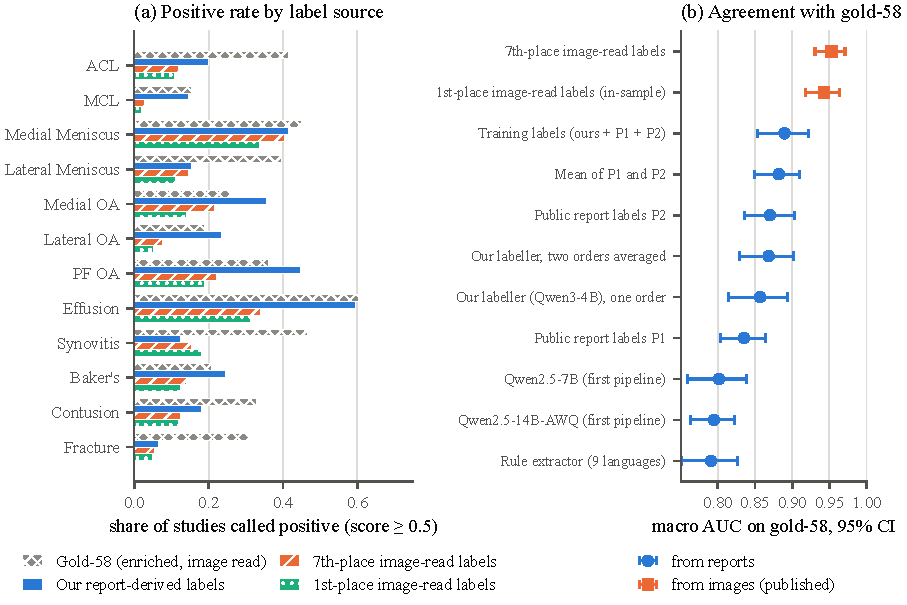
\includegraphics[width=\textwidth]{fig_labels.pdf}
\caption[Label prevalence and agreement with gold-58]{Label quality: (a) share of studies called positive by each label source (gold-58 is enriched, so its rates are not population rates), and (b) macro AUC of each label source against the gold-58 labels with 95\% bootstrap confidence intervals}
\label{fig:labels}
\end{figure}

\subsubsection{The forced-choice labeller} The new labeller follows the design of Section~\ref{sec:design-labels}. It runs Qwen3-4B-Instruct-2507 in 4-bit NF4 on the laptop GPU and reads the full report after Unicode normalisation and the Greek character repair. The prompt was developed on 60 non-gold studies and frozen before its first evaluation on gold. Two engineering problems had to be solved to make it fast enough. First, the Transformers library computes output logits over the whole vocabulary for every prompt position by default, which for an 8,000-token prompt needed 3.6~GB and pushed the card into shared system memory; asking for the logits of the last position only removed the problem. Second, the long system prompt is identical for every report, so its key--value cache was computed once and reused, which made the labeller about twelve times faster. On 96 test items the cached and uncached versions gave the same answers except for near-ties. The final labeller processed 0.94--1.6 studies per second with a peak of 4.4~GB of GPU memory, and each full pass over the 4,407 reports took about 75 minutes. All 4,407 reports were processed without a single failure, and the probability mass on the five answer letters was at least 0.995 everywhere. A rule-based extractor with negation handling for all nine languages was written as well, mainly to give an independent second opinion and evidence spans.

\subsubsection{Label quality against gold} Figure~\ref{fig:labels}(b) shows the macro AUC of every label source against the 58 gold studies. The forced-choice labeller scored 0.857, against 0.802 for the first Qwen2.5-7B pipeline; the paired difference was $+0.055$ with a 95\% confidence interval of $[+0.012, +0.093]$. Averaging its two item orders raised it to \textbf{0.868}, which is the score of our own labeller. The training labels of Equation~\eqref{eq:teacher}, the mean of our labeller and the public sets P1 and P2, reached 0.890 $[0.853, 0.922]$, the best of all report-based sources. As noted in Section~\ref{sec:design-labels}, part of P1 matches the gold labels exactly, so this figure may be slightly optimistic. The rule extractor was the weakest source at 0.791 and was not used for training. Every labeller had its lowest AUC on synovitis (0.67--0.74), and the strongest labellers called about two thirds of the gold-negative effusions positive. Both patterns come from differences between the reports and the images, which no report reader can fix.

\subsubsection{Effect of the labels on the image model} To answer this, the frozen-feature model of version~2 was retrained from scratch on each label set, with fixed epochs, five seeds, and gold used only for the final score. Table~\ref{tab:downstream} shows the result. Training on report-derived labels gave 0.75--0.78 on gold, while training on the 58 gold studies alone gave only 0.51--0.59. The labels were clearly useful. But the differences between label sets were small, within about 0.03, and masking the ``not mentioned'' cells made results worse. With frozen features the image model limited the result more than the labels did, so Stage~3 focused on the image model.

\begin{table}[htbp]
\centering\footnotesize\setstretch{1}
\caption[Downstream test of label sets with frozen features]{Downstream test: the frozen-feature model retrained on different label sets, scored on gold-58 (mean of five seeds)}
\label{tab:downstream}
\begin{tabular}{L{8.8cm}C{4.2cm}}
\toprule
Training labels & Gold-58 macro AUC [95\% CI] \\
\midrule
Final teacher (order-averaged LLM + two public sets) & 0.782 [0.735, 0.827] \\
Consensus of the first pipeline & 0.772 [0.725, 0.818] \\
Qwen2.5-7B labels of the first pipeline & 0.761 [0.709, 0.812] \\
Final teacher with ``not mentioned'' cells masked & 0.758 [0.707, 0.804] \\
Rule extractor & 0.747 [0.695, 0.798] \\
The 58 gold studies only (leave-one-out) & 0.51--0.59 \\
\bottomrule
\end{tabular}
\end{table}

% ----------------------------------------------------------------------
\subsection{Stage 3: The fine-tuned 2.5D multiple-instance model}
\label{sec:impl-mil}

\subsubsection{Pipeline corrections} The design of Section~\ref{sec:design-mil} was implemented as a set of Python modules for study indexing, decoding, data loading, the model, training and prediction. Before training, the defects of Table~\ref{tab:defects} that concern images were fixed and tested:
\begin{itemize}[leftmargin=1.4em]
\item \emph{Laterality.} The side is now taken from the tag or, failing that, from the coronal and axial geometry; disagreements between tag and geometry fell from 57 to 28 studies. After normalisation, the correlation between the mean left-knee image and the mean right-knee image rose from 0.869 to 0.988 in the coronal plane and from 0.950 to 0.988 in the sagittal plane.
\item \emph{Decoding.} A series that fails to decode falls back to the next candidate or is masked; it is never filled with zeros. A single unreadable slice at either end of a long series is dropped and recorded. If more than 2\% of the studies fail, the run stops.
\item \emph{Kaggle environment.} Kaggle's image used Python 3.13, for which no decoder wheels had been prepared, and pydicom finds its decoder plug-ins only at its first import. Without a fix, every compressed test study would have been decoded to nothing. We shipped decoder wheels for Python 3.10--3.14 in a private dataset and installed them before the first import of pydicom; the notebook checks for all four decoders before it starts.
\item \emph{Parity.} The preprocessing used for training and for inference was shown to give bit-identical arrays on 51 local series.
\end{itemize}

\subsubsection{Training} All training of this model ran on the laptop. The recipe is summarised in Table~\ref{tab:milrecipe}. One run of eight epochs on the four training folds (3,479 studies) took about 57 minutes at a steady 8.4 studies per second, with a peak of 3.8~GB of GPU memory. Long runs heated the GPU to its thermal limit and reduced its clock from about 3.1 to 2.0~GHz, and all timings in this report are at that throttled speed. Each run saved a complete checkpoint every epoch and could be resumed after the laptop slept or restarted.

\begin{table}[htbp]
\centering\footnotesize\setstretch{1}
\caption{Training recipe of the 2.5D multiple-instance model}
\label{tab:milrecipe}
\begin{tabularx}{\textwidth}{L{4.0cm} Y}
\toprule
Item & Setting \\
\midrule
Input & 3 series (sagittal, coronal, axial; fluid-sensitive first) $\times$ 8 windows $\times$ 3 slices, 224 $\times$ 224 pixels \\
Encoder & ConvNeXt-Tiny, ImageNet-22k pretrained and ImageNet-1k fine-tuned; drop-path 0.1 \\
Head & projection to 384 dimensions, slot and position embeddings, 12 attention heads, 12 linear outputs (28.4~M parameters in total) \\
Labels and loss & soft teacher labels (Equation~\ref{eq:teacher}), binary cross-entropy (Equation~\ref{eq:bce}); gold studies excluded \\
Optimiser & AdamW, learning rate $1\times10^{-4}$ for the encoder and $5\times10^{-4}$ for the head, weight decay 0.05 \\
Schedule & 0.5 epoch linear warm-up, cosine decay to zero at epoch 8; gradient-norm clipping at 1.0 \\
Batch & 2 studies with 2 accumulation steps (effective batch of 4 studies) \\
Precision and EMA & bfloat16 autocast on the laptop, float16 on T4; EMA decay 0.999 \\
Augmentation & one affine transform per series (rotation $\pm10^\circ$, scale $\pm10\%$, shift $\pm6\%$), gamma $\pm20\%$, gain $\pm10\%$, random window centres; no left--right flips, which would undo the laterality normalisation \\
\bottomrule
\end{tabularx}
\end{table}

\subsubsection{Results on the held-out fold} Figure~\ref{fig:curves}(a) shows the validation curves. Fine-tuning the encoder (run E1) reached a macro AUC of \textbf{0.882} $[0.873, 0.891]$ on the 870 studies of our fold~0, against 0.792 for the frozen-feature design re-run under the same protocol (E0, best of its three seeds; Figure~\ref{fig:curves}a shows their mean). The paired gain was $+0.090$ $[+0.079, +0.101]$, and every one of the twelve findings improved. It was the largest gain from any change to our own model. E0 was trained on our four training folds only and without averaging over seeds, which is why its gold score below (0.753) is lower than the 0.782 of the same frozen design in Table~\ref{tab:downstream}.

\begin{figure}[htbp]
\centering\setstretch{1}
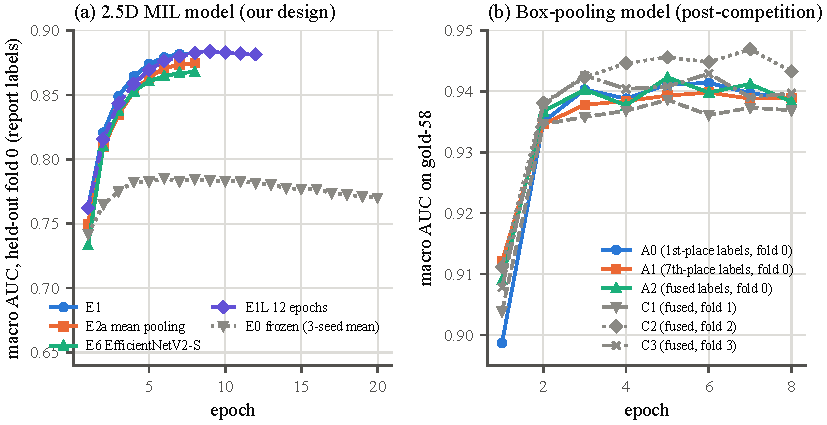
\includegraphics[width=\textwidth]{fig_curves.pdf}
\caption[Validation curves of the 2.5D and box-pooling models]{Validation curves: (a) our 2.5D model and its variants on our fold 0, scored against report-derived labels (E0 is the mean of three seeds); (b) the post-competition box-pooling runs on gold-58}
\label{fig:curves}
\end{figure}

\subsubsection{Ablations} We then tested one change at a time against E1, with the decision rule written down before the results were seen. Figure~\ref{fig:ablation} shows the paired differences on the held-out fold and on gold-58. A second run of the unchanged recipe with another seed differed from E1 by $+0.003$ on the held-out fold and by $+0.013$ on gold, which sets the scale of noise. Against that scale, none of the seven design changes was a clear improvement. A transformer layer over the tokens added $+0.002$ at 1.17 times the cost, and six series instead of three, a finer 0.6~mm pixel grid and twelve epochs made no clear difference. Mean pooling ($-0.008$), confidence-weighted labels ($-0.005$) and an EfficientNetV2-S encoder \cite{tan2021effnetv2} ($-0.015$) were worse, and on gold-58 all three pointed the same way. The eighth row of the figure, E1p, is a bug fix described below. The design of Section~\ref{sec:design-mil} was therefore kept as it was.

\begin{figure}[htbp]
\centering\setstretch{1}
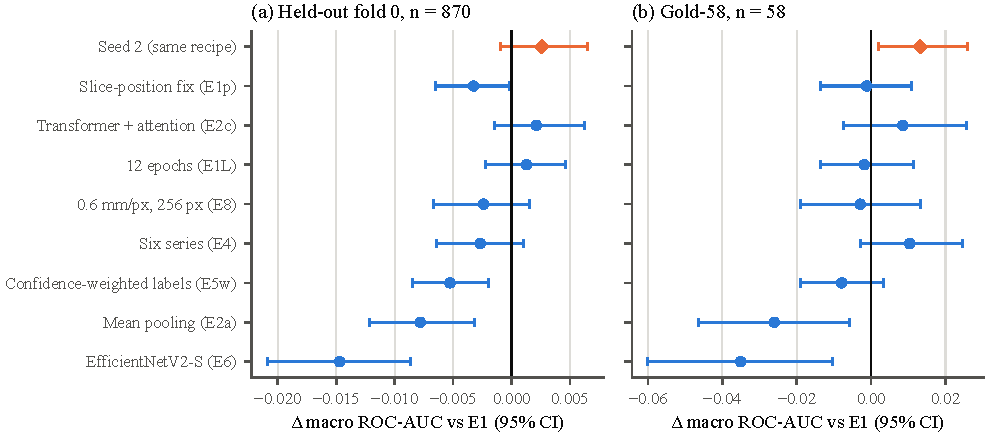
\includegraphics[width=\textwidth]{fig_ablation.pdf}
\caption[Single-change ablations of the 2.5D model]{Single-change ablations of the 2.5D model, as paired differences in macro AUC from run E1: (a) on the 870 studies of our fold 0 and (b) on gold-58; the orange point is a second seed of the unchanged recipe and shows the noise level}
\label{fig:ablation}
\end{figure}

\subsubsection{Where the model looks} Because each finding has its own attention distribution, the attention weights show where the model gathers its evidence, even though it was never told where any finding is. We averaged them over 300 validation studies (Figure~\ref{fig:attention}). The MCL head puts half of its weight on the coronal plane, where the collateral ligaments are seen along their length. The Baker's cyst head prefers coronal and axial slices, and the effusion head the axial plane. In the sagittal plane, the lateral meniscus head looks at the lateral end of the stack (mean position 0.39) and the medial meniscus head at the medial end (0.64). This separation can only appear if the laterality normalisation works. The same analysis exposed one more defect. The slice-position input was mirrored for right-knee sagittal series. It was fixed (run E1p) and the fix was kept as a correctness change; its effect on the score ($-0.003$) was no larger than the difference between two seeds.

\begin{figure}[htbp]
\centering\setstretch{1}
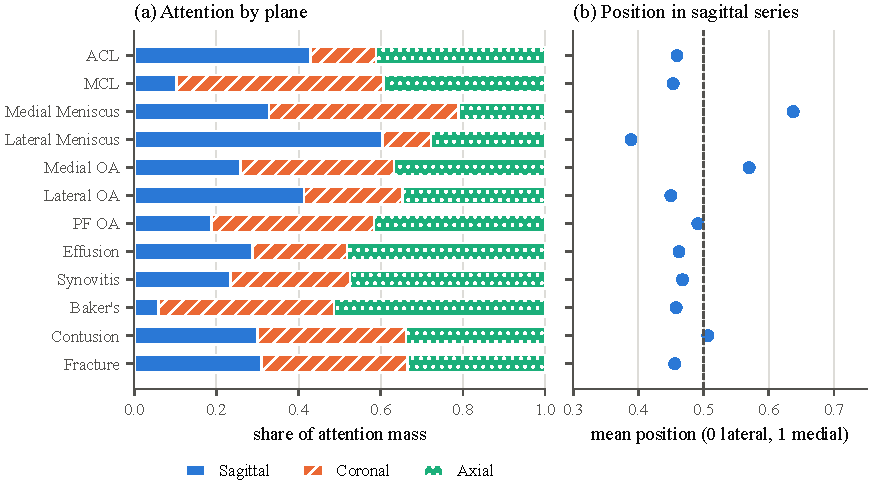
\includegraphics[width=\textwidth]{fig_attention.pdf}
\caption[Attention of the 2.5D model by plane and position]{Where the per-finding attention of the 2.5D model goes, averaged over 300 validation studies: (a) share of the attention on each plane and (b) mean position of the attention within the sagittal series}
\label{fig:attention}
\end{figure}

\subsubsection{Test-time averaging and the final ensemble} Larger sets of windows at test time did not help, but averaging two sets of eight windows, the second shifted by half a step, gave a small consistent gain of $+0.0017$ $[+0.0001, +0.0033]$ and was adopted. The final package contained three models with the locked recipe, F1, F2 and F3, trained with seeds 42, 7 and 11 on all 4,349 report-labelled studies (84--86 minutes each). Only after this choice was fixed was gold-58 scored, once, for all runs together. The final ensemble reached \textbf{0.906} $[0.877, 0.932]$ on gold-58, against 0.753 for the frozen-feature design (Figure~\ref{fig:gold}). Synovitis was the clear outlier at 0.680, close to the 0.68--0.74 of the report labels themselves. The model had learned what the reports say about synovitis rather than what the images show.

\begin{figure}[htbp]
\centering\setstretch{1}
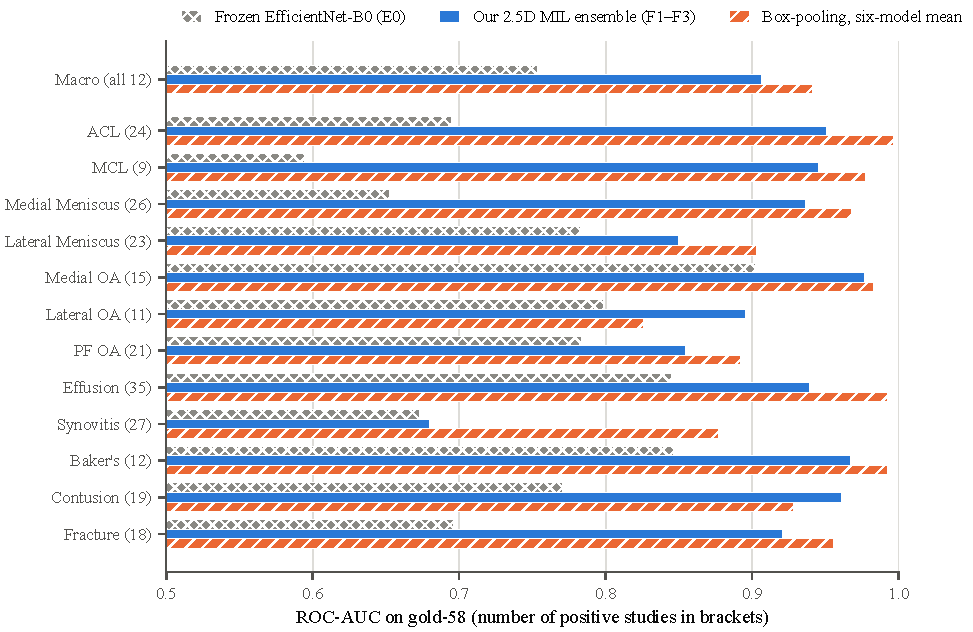
\includegraphics[width=\textwidth]{fig_gold_per_finding.pdf}
\caption[Per-finding AUC on gold-58]{Per-finding AUC on gold-58 for the frozen-feature baseline, our final 2.5D ensemble (Stage 3) and the six-model box-pooling ensemble (Stage 5)}
\label{fig:gold}
\end{figure}

\subsubsection{Submission} Measured end to end on the laptop, the three-model package with test-time averaging needed 1.9~s per study, about 42 minutes for 1,300 studies, of which 70--80\% was DICOM reading and decoding. The submission scored \textbf{0.927 on the public leaderboard and 0.916 on the private leaderboard}. A later variant added a fourth model, E9, trained at higher resolution (0.365~mm per pixel with a 320-pixel crop). It had gained $+0.005$ $[+0.001, +0.009]$ on the held-out fold, which is within the 0.003--0.006 differences we had seen between repeated runs of the same recipe, and on the leaderboard it scored 0.928 public and 0.915 private, the same as before. A round of self-training on the model's own out-of-fold predictions was also trained but never scored on the leaderboard, so we make no claim about it.

% ----------------------------------------------------------------------
\subsection{Stage 4: The competition endgame}
\label{sec:impl-endgame}

\subsubsection{The gap} With five days left, the best public notebooks scored 0.954--0.958 on the public leaderboard against our 0.927. Every public notebook above 0.950 used a CoAtNet \cite{dai2021coatnet} model that its author had trained with 2,399 additional knees from the OAI \cite{nevitt_oai,nartaa_swa}. Our own experiments in Stage~3 had found no change to our model that moved the held-out score beyond noise, and closing a gap of 0.03 with a single model of our own in five days was not realistic. We therefore changed strategy for the final submissions. Instead of one model of our own, we built ensembles around the strongest public models (Table~\ref{tab:public}) and spent our effort on checking, combining and re-engineering them.

\begin{table}[htbp]
\centering\footnotesize\setstretch{1}
\caption[Public models used in the competition endgame]{Public models and notebooks used in the competition endgame, with the extra data in their training as traced by us and their macro AUC when we ran them on gold-58}
\label{tab:public}
\begin{tabularx}{\textwidth}{L{2.0cm} L{2.6cm} Y C{1.3cm} L{2.6cm}}
\toprule
Model & Published by & Network and extra training data & Gold-58 & Used in \\
\midrule
CoAtNet & nartaa \cite{nartaa_swa} & CoAtNet at 384 pixels; 2,399 extra knees from the OAI & 0.923 & every pick \\
S6 & heliosli \cite{heliosli_compact} & ConvNeXt with an anatomy crop model trained on SKM-TEA & 0.927 & A-strict, final-strict \\
s6fall & nartaa \cite{nartaa_s6fall} & S6 retrained on all report-labelled studies & 0.931 & final-strict, final-max \\
R6 & heliosli, re-hosted by rostigor \cite{rostigor_r6} & ConvNeXt at 384 pixels with the same SKM-TEA crop model; auxiliary task on fastMRI+ (inferred from its trainer) & 0.937 & final-max \\
\midrule
\multicolumn{5}{L{15.6cm}}{Notebooks used as the base of our picks: heliosli's CoAtNet + S6 blend \cite{heliosli_blendgold} (A-strict) and goodpjw2008's CoAtNet + R6 pipeline \cite{goodpjw_coatnet_nb} (final-max).} \\
\bottomrule
\end{tabularx}
\end{table}


\subsubsection{Provenance checks} External data was allowed only if it was freely and equally available. We traced the training data of every public model we considered. The CoAtNet models used the OAI, which needs only a registration and a click-through data-use agreement; in our reading this met the organisers' general test, although they gave no ruling on individual datasets. A model called R6 and its successor R7 turned out to use an auxiliary task trained on fastMRI+ \cite{zhao2022fastmriplus}, whose access requires an institutional affiliation. The crop model of another family used SKM-TEA \cite{desai2021skmtea}. One of the two final picks was kept free of fastMRI-derived models, so that the team had one entry that did not depend on that question.

\subsubsection{Running every model ourselves} Before any model went into a submission, we ran it on the laptop with its author's code and scored it on gold-58 (Table~\ref{tab:public}). This needed some porting. One fast DICOM reader used a system call that exists only on Unix; on Windows the error was swallowed and every volume came back empty without any message. We patched the reader, checked that its output was byte-identical to the original on a reference set, and added a check that every volume contains slices. The local runs also gave us the cost of each model, which decided what could fit in the nine-hour limit: about 3~s per study for the CoAtNet, 6.5~s for s6fall, 19~s for S6 and 54--62~s for R6, which runs four folds with mirrored copies.

\subsubsection{Designing the blends} The ensembles themselves were ours. For each submission we fixed the members and their weights in writing before it was scored. The fastMRI-free pick, final-strict, combines the CoAtNet, S6 and s6fall with weights 0.5, 0.25 and 0.25; before it ran we predicted 0.955--0.956 on the public leaderboard, and it scored 0.956. For A-strict+ we replaced the R6 stage of the strongest public notebook with S6 and added a second, 224-pixel CoAtNet checkpoint inside the CoAtNet share and a 2.5D reader at one tenth of the weight. We then tested six further blend upgrades on gold-58, again with an adoption rule fixed in advance, among them standardised logits, per-compartment weights and mirrored test-time averaging, and separately a small calibration adapter. None passed. Mirrored averaging, for example, lowered S6 by 0.0066 $[-0.0107, -0.0026]$ on 300 held-out studies, each scored by a fold model that had never seen it.

\subsubsection{Fitting an extra model into the time limit} The strongest public notebook \cite{goodpjw_coatnet_nb} already needed 6.5--8 hours on the hidden test, so a model added as a separate stage, which decodes every study again, could never finish within nine hours. We rewrote the inference worker so that the added model scores a second rendering of each study inside the existing decode pass, at its own resolution of 320 pixels next to R6's 384. On the first gold study the rewritten stage matched the separate stage to $2\times10^{-10}$, and over all 58 gold studies the two agreed on 57; the remaining study was the one whose knee side was decided differently.

\subsubsection{Fine-tuning on our labels} We also fine-tuned the public s6fall model on our own labels, on the 6~GB laptop GPU. We first built a cache of every slice window of the 4,349 studies (about 150~GB, written in about three hours) and then wrote a trainer that freezes the first two stages of the encoder, uses gradient checkpointing and bfloat16, and trains on one study at a time with gradient accumulation, which kept the peak memory at 2.3~GB. The loss combined soft binary cross-entropy with a pairwise ranking term, since the metric is a ranking measure, and an EMA of the weights was kept. The first fine-tune (three epochs, about four hours) scored 0.928 on gold-58 against 0.931 for the model it started from. For the second we rebuilt the targets with the out-of-fold predictions of S6 as an extra teacher; it reached 0.937, but in the blends its gain was $+0.0007$ to $+0.0010$ with confidence intervals that crossed zero. Neither fine-tune passed our adoption rule or entered the final picks. Both were later tried in submissions 10 and 11, which scored the same as the blends without them.

\subsubsection{Submissions and final result} Table~\ref{tab:endgame} lists the main submissions of this stage, and Figure~\ref{fig:leaderboard} shows all of our submissions in order. The fastMRI-free blend (``final-strict'') scored 0.956 public, and the blend including R6 (``final-max'', version~2 with the single-pass rewrite) scored 0.958 public. These two were chosen as the final picks.

\begin{table}[htbp]
\centering\footnotesize\setstretch{1}
\caption[Main submissions of the competition endgame]{Main submissions of the competition endgame (public / private leaderboard macro AUC)}
\label{tab:endgame}
\begin{tabularx}{\textwidth}{L{2.7cm} Y C{1.25cm} C{1.25cm}}
\toprule
Submission & Content & Public & Private \\
\midrule
A-strict & public CoAtNet (OAI) + public S6, weights 0.7/0.3 \cite{heliosli_blendgold} & 0.954 & 0.937 \\
A-strict+ & public 0.958 notebook with its R6 stage replaced by S6 & 0.954 & 0.937 \\
final-strict & A-strict + public s6fall (0.5/0.25/0.25); fastMRI-free; \textbf{final pick} & 0.956 & 0.940 \\
final-max v1 & public CoAtNet + R6 notebook + s6fall as a separate stage & 0.958 & 0.943 \\
final-max v2 & as v1, s6fall scored inside the R6 decode pass; \textbf{final pick} & 0.958 & 0.943 \\
final-max v3 & v2 + our two fine-tuned models (not adopted by our rule) & 0.958 & 0.943 \\
last-day variants & per-finding blend weights fitted on gold-58; at least one stopped at its time limit & 0.848--0.948 & 0.850--0.935 \\
\bottomrule
\end{tabularx}
\end{table}

\begin{figure}[htbp]
\centering\setstretch{1}
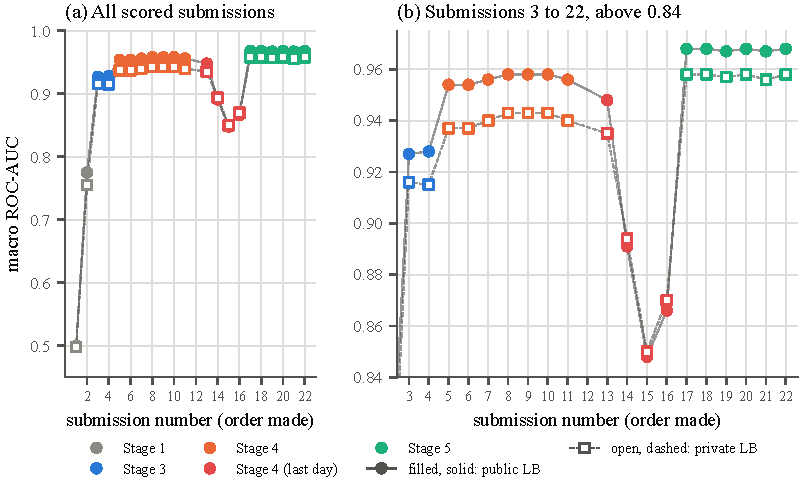
\includegraphics[width=\textwidth]{fig_leaderboard.pdf}
\caption[Leaderboard scores of all submissions]{Every submission made from the team's account, in order, with its public (filled) and private (open) score; stages as in Figure~\ref{fig:stages}, and submission 12 returned no score}
\label{fig:leaderboard}
\end{figure}

Several submissions of the last day scored lower than the picks. For these we relaxed our adoption rule and fitted separate blend weights for each finding on the 58 gold studies, which raised the gold score of the blend from 0.939 to 0.954. That gain was measured on the same 58 studies the weights were fitted to, so it was in-sample and meant little. For the same submissions we also fine-tuned the CoAtNet model for two epochs on Kaggle's GPUs (gold-58 0.924 against 0.923 before). To make room for more models, the blends also ran closer to the time limit. The results ranged from 0.948 down to 0.848 on the public leaderboard. For one of them the cause is known. It reached its internal deadline of 8.3 hours, and every study it had not reached received a constant default value. For the others the hidden-test logs are not visible to participants, so the cause could not be confirmed. None of these submissions was selected.

The team's final private score was \textbf{0.943}, from the better of the two picks, final-max v2, which contains R6; the fastMRI-free pick scored 0.940. This placed the team 490th of 6,299 teams on the private leaderboard, which earned a bronze medal; Kaggle's certificate is reproduced in Appendix~\ref{app:certificate}. The winning private score was 0.960. Our picks lost 0.015 between the public and the private leaderboard, against 0.010--0.011 for our own Stage~3 model and the later box-pooling model. The extra loss is consistent with, but does not prove, overfitting of the public blends to the public leaderboard.

% ----------------------------------------------------------------------
\subsection{Stage 5: Post-competition diagnosis and the improved model}
\label{sec:impl-post}

After the competition closed, the top teams published their methods and some of their code and labels. This made it possible to test, with controlled experiments, why our own model had stopped at 0.916 private.

\subsubsection{What the top solutions had in common} We read twelve published solutions. Their main points of agreement were: (1) labels made by LLM agents that look at the images as well as the report scored 0.93--0.95 against gold-58, far above our 0.890; (2) cropping and pooling each finding inside an anatomical region of interest added a further gain; (3) large ensembles added little; and (4) a single well-built model reached 0.954--0.958 on the private leaderboard. The first- and seventh-placed teams published their image-read labels \cite{tascj_agentlabels,songqizhou_llmlabels}, and the first-placed team also published its complete training code \cite{tascj_boxpool,tascj_roidetector,tascj_sideclassifier}.

\subsubsection{Measuring our labels} Figure~\ref{fig:labels}(a) compares our labels with the two image-read sets on the same 4,349 studies. Our report labels call MCL injury in 14.7\% of the studies against 2--3\% for the image readers, lateral OA in 23.5\% against 5--8\%, PF OA in 44.6\% against 19--22\%, and effusion in 59.4\% against 31--34\%. Reports mention small effusions and mild degenerative changes that an image reader working to a threshold would call negative. Against gold-58 the seventh-place labels scored 0.953 and the first-place labels 0.943; the latter were partly fitted to gold, so their score is in-sample (Figure~\ref{fig:labels}b). The two image-read sets disagree with each other on 1--10\% of the studies per finding, most often on synovitis (9.7\%), medial OA (8.9\%) and the medial meniscus (8.7\%).

\subsubsection{The label-swap experiment} To measure the effect of labels alone, we retrained our exact Stage~3 recipe (same fold, same seed, same code) and changed only the label file. Figure~\ref{fig:labelswap}(a) shows the result on gold-58. With our report labels the model scored 0.891; with the first-place labels 0.912 ($+0.021$, CI $[+0.004, +0.039]$); with the seventh-place labels 0.927 ($+0.036$, CI $[+0.018, +0.055]$); and with the mean of the two image-read sets 0.928. Synovitis alone rose from 0.689 to 0.857 with the seventh-place labels. Both gains were confirmed on our fold~0, where each model was scored against the image-read label set it had not been trained on: $+0.029$ and $+0.026$ over the model trained on our labels. This answers the question left open in Stage~2. Once the encoder was fine-tuned, the labels limited our model more than its design did.

\begin{figure}[htbp]
\centering\setstretch{1}
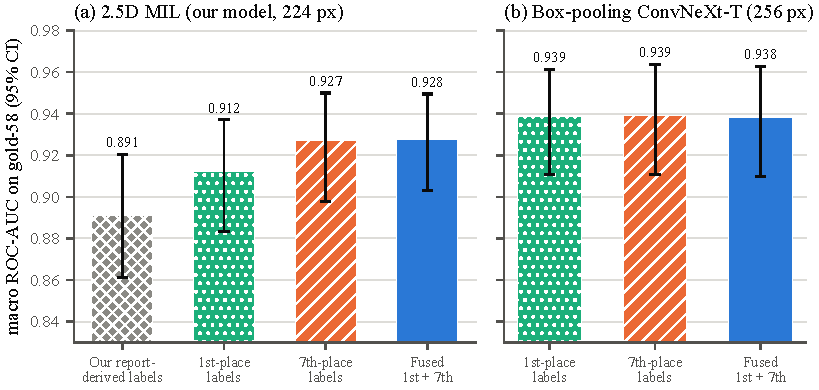
\includegraphics[width=\textwidth]{fig_label_swap.pdf}
\caption[Label-swap experiment on gold-58]{Label-swap experiment on gold-58 (95\% bootstrap CI): (a) our 2.5D model retrained with only the label file changed; (b) the box-pooling model trained with the same three image-read label choices}
\label{fig:labelswap}
\end{figure}

We also re-scored all the Stage~3 ablations against the image-read labels. The seed-to-seed spread on our fold~0 was about 0.007, and the higher resolution, six series, twelve epochs and the transformer head were all inside it. EfficientNetV2-S ($-0.018$) and mean pooling ($-0.013$) were worse by more than that spread. Under the image-read labels the higher-resolution version of our model (320-pixel crop, 0.365~mm per pixel) gained only $+0.003$ $[+0.001, +0.006]$ on our fold~0 and nothing on gold-58 (0.927 against 0.927), at 1.7 times the training time, so resolution was not pursued. An idea of our own, centring the predicted scores within each scanner group, lowered the score on our fold~0 from 0.926 to 0.917 and was dropped.

\subsubsection{Adopting the box-pooling architecture} With the image-read labels our model reached 0.927 on gold-58, roughly where the first-placed team's write-up places its own model before region-of-interest pooling, cropping and the auxiliary heads. Rebuilding those parts ourselves would have taken longer than the time available before the project presentation. We therefore adopted their published architecture (Section~\ref{sec:design-bp}) as the base and focused our own work on the labels, the training plan, the inference pipeline and the evaluation.

\subsubsection{Training on Kaggle} We wrote a builder that generates a training notebook from the published script with switches for the label file, fold, seed and time budget. It also saves validation predictions for every series and adds an inference-only switch for attention sharpening, described below. The runs used the free two-T4 quota of a team member's Kaggle account. Each run trained for eight epochs on about 19,200 series (2,400 updates per epoch) and took 5.4--6.1 hours of training, plus validation. The data loader waited only 1\% of the time while reading directly from Kaggle's network storage, so no image cache was needed. Six runs were made (Table~\ref{tab:bpruns}), all on the five-fold split of the published code. A0 and A1 differ only in the label set, A2 uses the fused labels of Equation~\eqref{eq:fused}, and C1--C3 repeat A2 on folds 1--3, so that the six models together cover different training subsets. Validation on gold-58 was recorded every epoch (Figure~\ref{fig:curves}b), but the last epoch was always used; gold was never used to choose an epoch.

\begin{table}[htbp]
\centering\footnotesize\setstretch{1}
\caption[Box-pooling training runs]{Box-pooling training runs (8 epochs each, Kaggle 2 $\times$ T4); gold-58 at the last epoch}
\label{tab:bpruns}
\begin{tabular}{C{1.1cm}L{4.4cm}C{1.1cm}C{2.0cm}C{2.4cm}}
\toprule
Run & Training labels & Fold & Gold-58 AUC & Training time (h) \\
\midrule
A0 & first-place image-read labels & 0 & 0.9388 & 5.5 \\
A1 & seventh-place image-read labels & 0 & 0.9389 & 5.7 \\
A2 & fused (mean of both) & 0 & 0.9383 & 5.4 \\
C1 & fused & 1 & 0.9369 & 5.7 \\
C2 & fused & 2 & 0.9433 & 6.1 \\
C3 & fused & 3 & 0.9397 & 5.6 \\
\midrule
\multicolumn{3}{l}{Mean of the six models} & 0.9409 & -- \\
\bottomrule
\end{tabular}
\end{table}

\subsubsection{Our inference pipeline} The published inference notebooks depended on TensorRT engines and a compiled reader tied to the authors' own weights, so we wrote our own inference script that runs the three published modules unchanged: side classifier, detector (with mirrored test-time averaging) and box-pooling classifiers. A series that cannot be read is skipped and reported, never filled with zeros. A series without detector boxes receives the median box of its plane, and a batch that fails, for example from running out of memory on a very long series, is repeated one series at a time. Locally it ran the three public test studies in 25~s, and on 16 gold studies its predictions matched the published notebook's own predictions for the same weights with a correlation of 0.996. Before any GPU time was spent, the notebook was rehearsed in a free CPU session on Kaggle with every multi-series batch forced to fail once; all 15 series were recovered by the one-at-a-time path and the run completed in 202~s.

\subsubsection{Results} The A0 versus A1 comparison was a tie: 0.9388 against 0.9389 on gold-58, and on the published fold~0 each model won by about 0.003 when scored against its own label source (Figure~\ref{fig:labelswap}b). The stronger architecture was much less sensitive to the label set than our own model had been, where the same swap had made a difference of 0.015. The fused labels gave a model between the two single-source models on every reference. Late submissions, which Kaggle scores on the private leaderboard but does not rank, gave the results in Table~\ref{tab:late}. Model A0, the published recipe trained unchanged on one fold, scored 0.955 private, which reproduces the 0.954 published for it and shows that our inference pipeline is sound. Training the same pipeline on the fused labels gave 0.958, a difference of the size that the leaderboard's own noise could produce. Every model or average of models trained on image-read labels scored 0.955--0.958 private, against 0.943 for our best submission during the competition and 0.960 for the winning team.

\begin{table}[htbp]
\centering\footnotesize\setstretch{1}
\caption[Late submissions of the box-pooling models]{Late submissions of the box-pooling models (scored after the competition, not ranked)}
\label{tab:late}
\begin{tabular}{L{6.3cm}C{2.0cm}C{2.0cm}L{2.6cm}}
\toprule
Models & Private & Public & Account \\
\midrule
A0 (first-place labels) & 0.955 & 0.963 & team member$^{*}$ \\
A1 (seventh-place labels) & 0.957 & 0.967 & team member$^{*}$ \\
A0 + A1 & 0.958 & 0.967 & team member$^{*}$ \\
A2 (fused labels) & 0.958 & 0.968 & both \\
A2 + C1 & 0.958 & 0.968 & team \\
A0 + A1 + A2 & 0.958 & 0.968 & team \\
A0 + A1 + A2 + C1 & 0.958 & 0.968 & team \\
A1 with attention sharpening $s=2$ & 0.956 & 0.967 & team \\
A1 with per-finding sharpening & 0.957 & 0.967 & team \\
\bottomrule
\multicolumn{4}{l}{\scriptsize $^{*}$ scores from the project's decision log; all other rows read from the Kaggle submission history.}
\end{tabular}
\end{table}

Before the last two folds were trained, we fixed in writing that the equal-weight mean of all six models would be reported as the final ensemble. This was done because picking the best of many variants by its leaderboard score would itself be a form of selection on the test set. The notebook for this six-model ensemble, built automatically when the last two runs finished, stopped with an error on Kaggle and was not scored at the time of writing. On gold-58 the six-model mean scores 0.941 $[0.912, 0.965]$, which we report as a description only. Figure~\ref{fig:gold} shows that it gains most on synovitis (0.877 against 0.680 for our Stage~3 model), effusion, ACL and the menisci, while our Stage~3 model remains better on lateral OA and bone contusion.

\subsubsection{Ideas that were tested and rejected} Four further ideas were examined on the published fold~0 before any leaderboard submission. Three were tested against a rule fixed in advance and one was only considered.
\begin{itemize}[leftmargin=1.4em]
\item \emph{Adding our own study-level model to the ensemble.} Trained with the published fold~0 held out, our model scored 0.957 alone against 0.968--0.971 for the box-pooling models, and adding it at one third weight changed the score by $-0.0012$ $[-0.0023, -0.0000]$. It was not added.
\item \emph{Attention sharpening.} Multiplying the in-box attention score $a$ of Equation~\eqref{eq:boxweight} by a factor $s$ at inference makes the pooling more ($s>1$) or less ($s<1$) focused. Two other teams had reported a gain from this in their own models. Figure~\ref{fig:sharpen} shows that the trained models already sit at their optimum: $s=1.25$ gained at most $+0.0007$, while $s=3$ lost 0.004--0.006. Focal findings such as medial OA and fractures gained slightly from sharpening, while diffuse findings, above all synovitis, lost. Two sharpened versions sent to the leaderboard as a check scored 0.956 and 0.957 private, against 0.957 for the unchanged model, so sharpening was not adopted.
\item \emph{Weighting series types.} Instead of the plain mean over a study's series, we fitted one weight per finding and series type (plane and fat suppression) with five-fold cross-fitting. The best setting gained $+0.0004$ to $+0.0007$, ten times smaller than the seed spread; with weaker regularisation the weights spread by a factor of 50 and the score fell. Fixed alternatives such as the maximum over series were worse, and the plain mean was kept.
\item \emph{Test-time flipping of the classifier.} Not tried for this model, because left knees are already mirrored before classification, and a related test in Stage~4 had lowered the score of a public model by 0.007.
\end{itemize}

\begin{figure}[htbp]
\centering\setstretch{1}
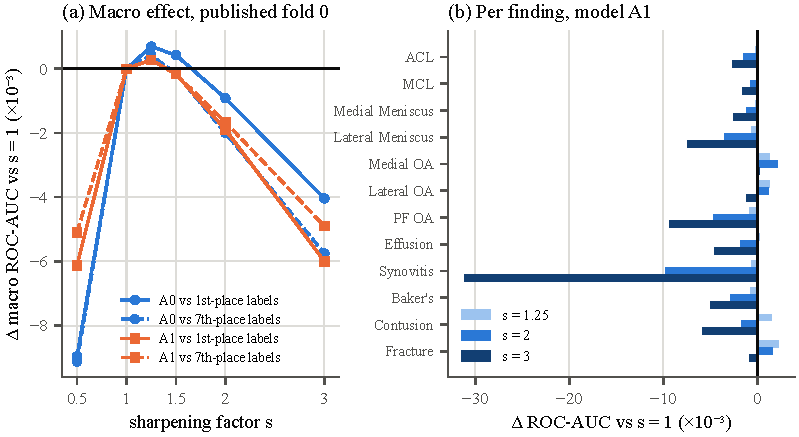
\includegraphics[width=\textwidth]{fig_sharpen.pdf}
\caption[Attention sharpening at inference]{Attention sharpening at inference on the 870 studies of the published fold 0: (a) change in macro AUC for models A0 and A1 scored against both image-read label sets; (b) change per finding for model A1 against the first-place labels}
\label{fig:sharpen}
\end{figure}

% ----------------------------------------------------------------------
\subsection{Stage 6: The local workstation}
\label{sec:impl-demo}

The last part of the project made the final models usable outside Kaggle. The workstation follows the design of Section~\ref{sec:design-demo}. A user drops a DICOM folder, a set of files or a zip archive onto the page. The browser packs the files and sends them to the local server, which parses the headers, groups the series, skips localisers and series with fewer than six slices, reads the fat-suppression setting from the header (it agreed with the dataset's own labels on 99\% of 600 training series) and places every slice in patient coordinates for the three-dimensional view. Inference then runs the side classifier, the detector and all six classifiers one series at a time and streams every intermediate result to the page as it is computed. Figure~\ref{fig:ws-overview} shows the screen after a run on one of the three public example test studies. The detector's box for the medial meniscus and the cells with positive evidence are drawn on the sagittal, coronal and axial views.

\begin{figure}[htbp]
\centering\setstretch{1}
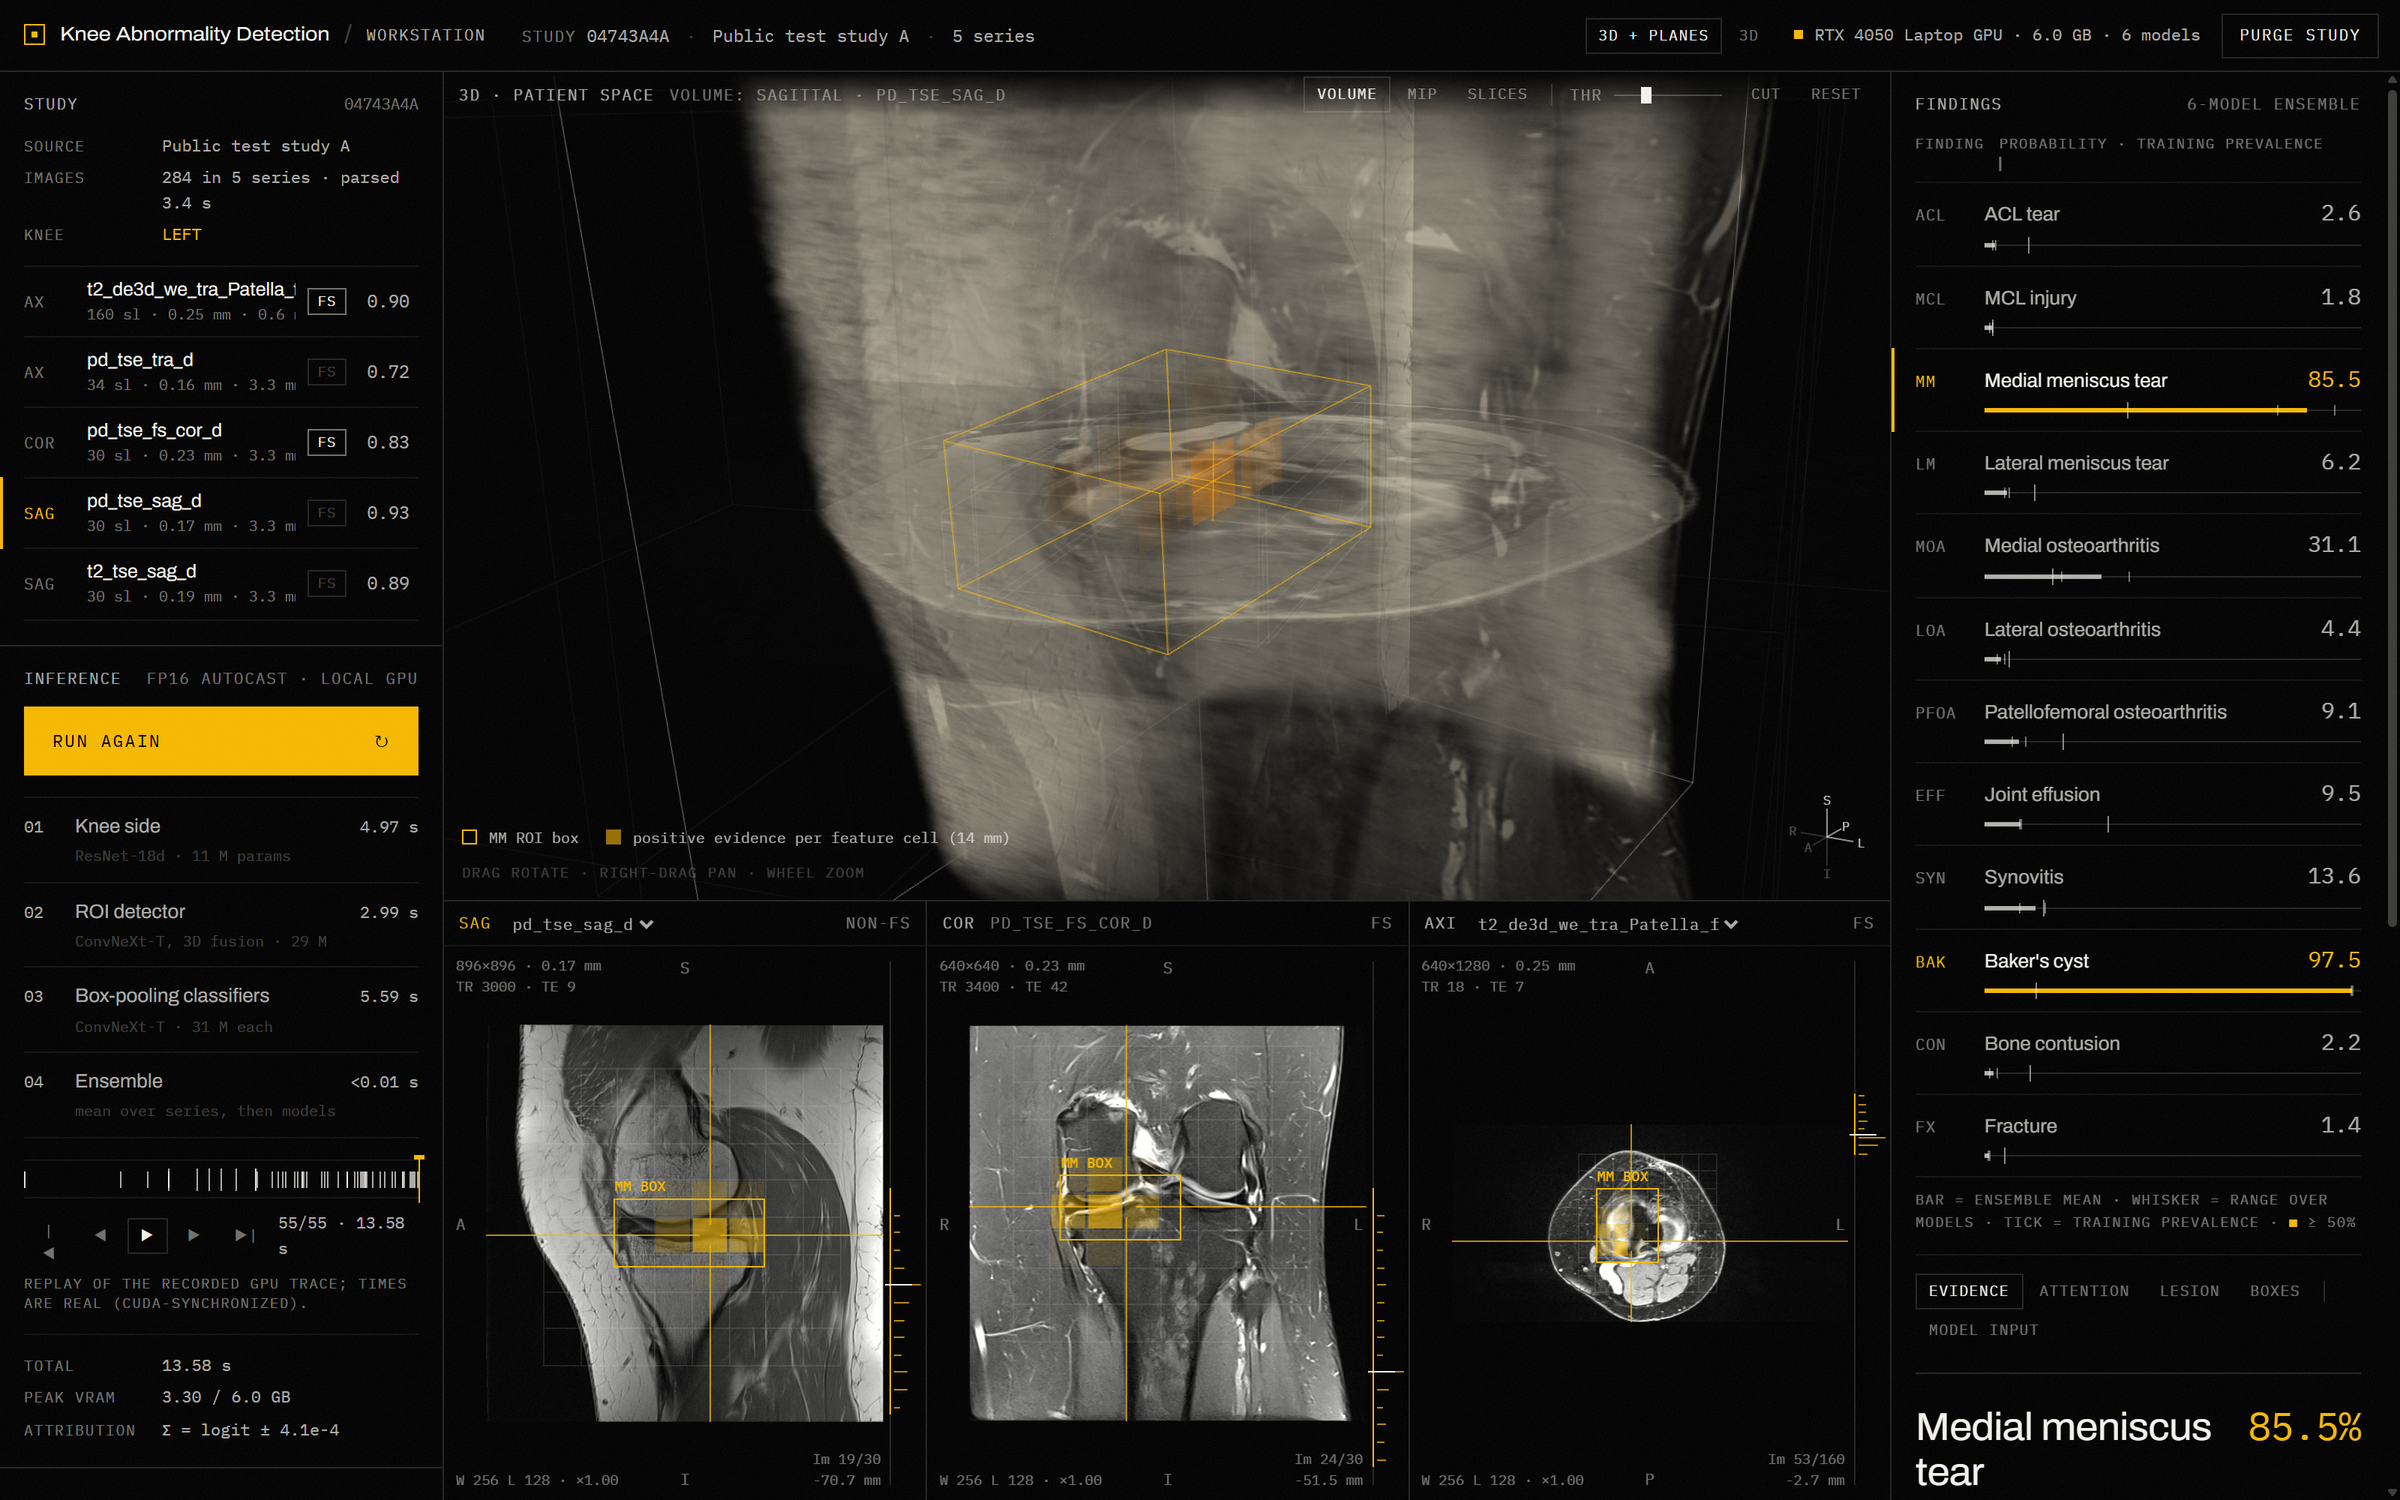
\includegraphics[width=\textwidth]{ws_overview.png}
\caption[The local workstation after inference]{The local workstation after inference on a public example study: series list and GPU trace on the left, the three-dimensional view and the three plane views with the medial meniscus box and evidence cells in the centre, the twelve findings with ensemble mean and model range on the right}
\label{fig:ws-overview}
\end{figure}

For each finding the page shows the ensemble probability, the spread across the six models, and the training prevalence for reference. Selecting a finding opens its detail panel (Figure~\ref{fig:ws-detail}b): the probability from each model, the probability from each series, and the slices that contributed most to the score. Four overlays can be laid over the images: the detector's box, the pooling weights, the evidence of Equation~\eqref{eq:attribution} averaged over the six models, and the output of the lesion head, which was trained to mark lesion cells but does not feed the probability, so it gives an independent second localisation. The panel states plainly that the evidence map shows what drove the score, which need not be the most visible lesion.

\begin{figure}[htbp]
\centering\setstretch{1}
\begin{minipage}[b]{0.40\textwidth}\centering
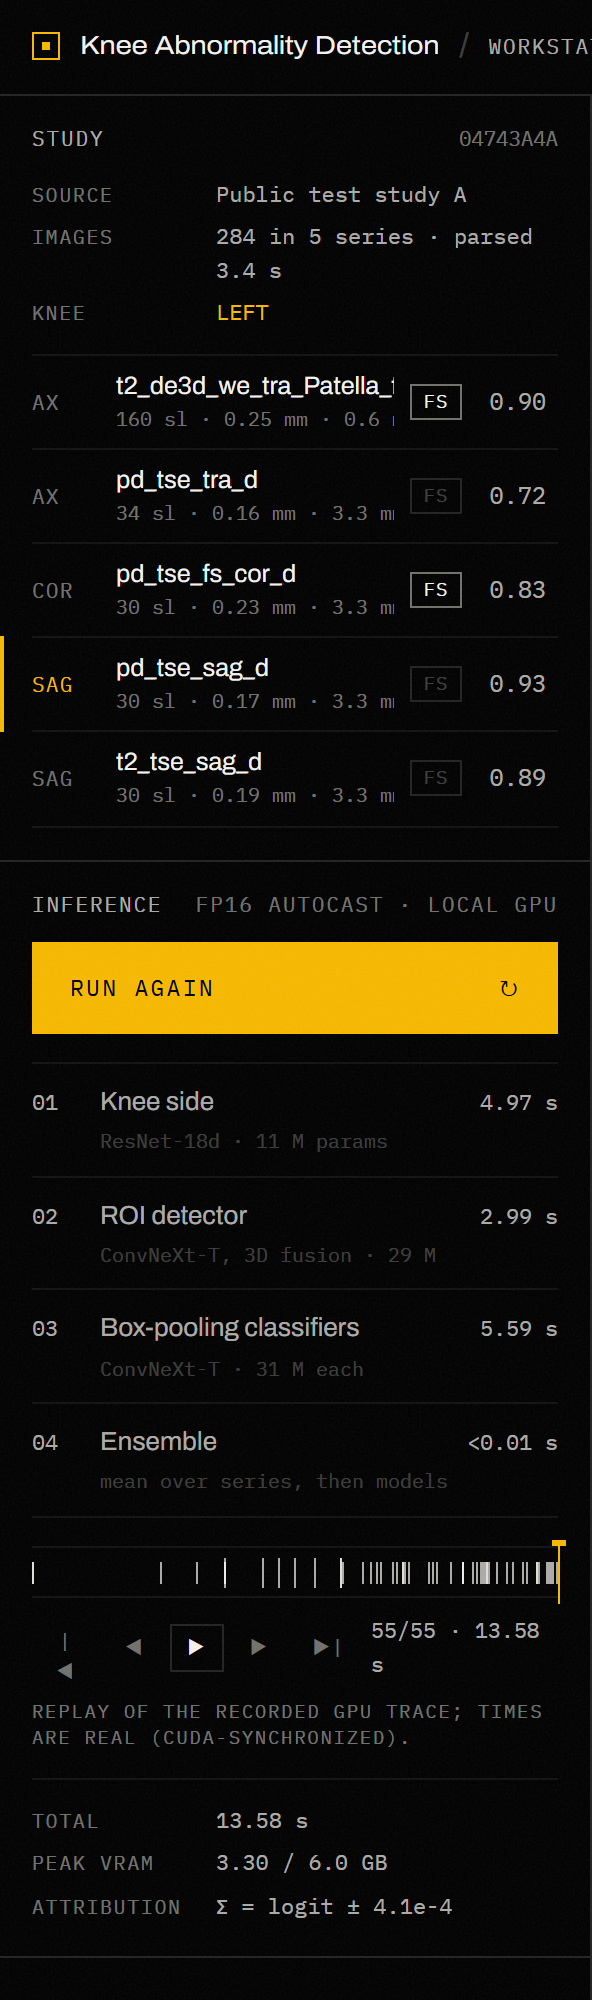
\includegraphics[height=16.5cm]{ws_left_panel.png}\\[2pt]
{\footnotesize\itshape (a) study, series and inference trace}
\end{minipage}\hfill
\begin{minipage}[b]{0.55\textwidth}\centering
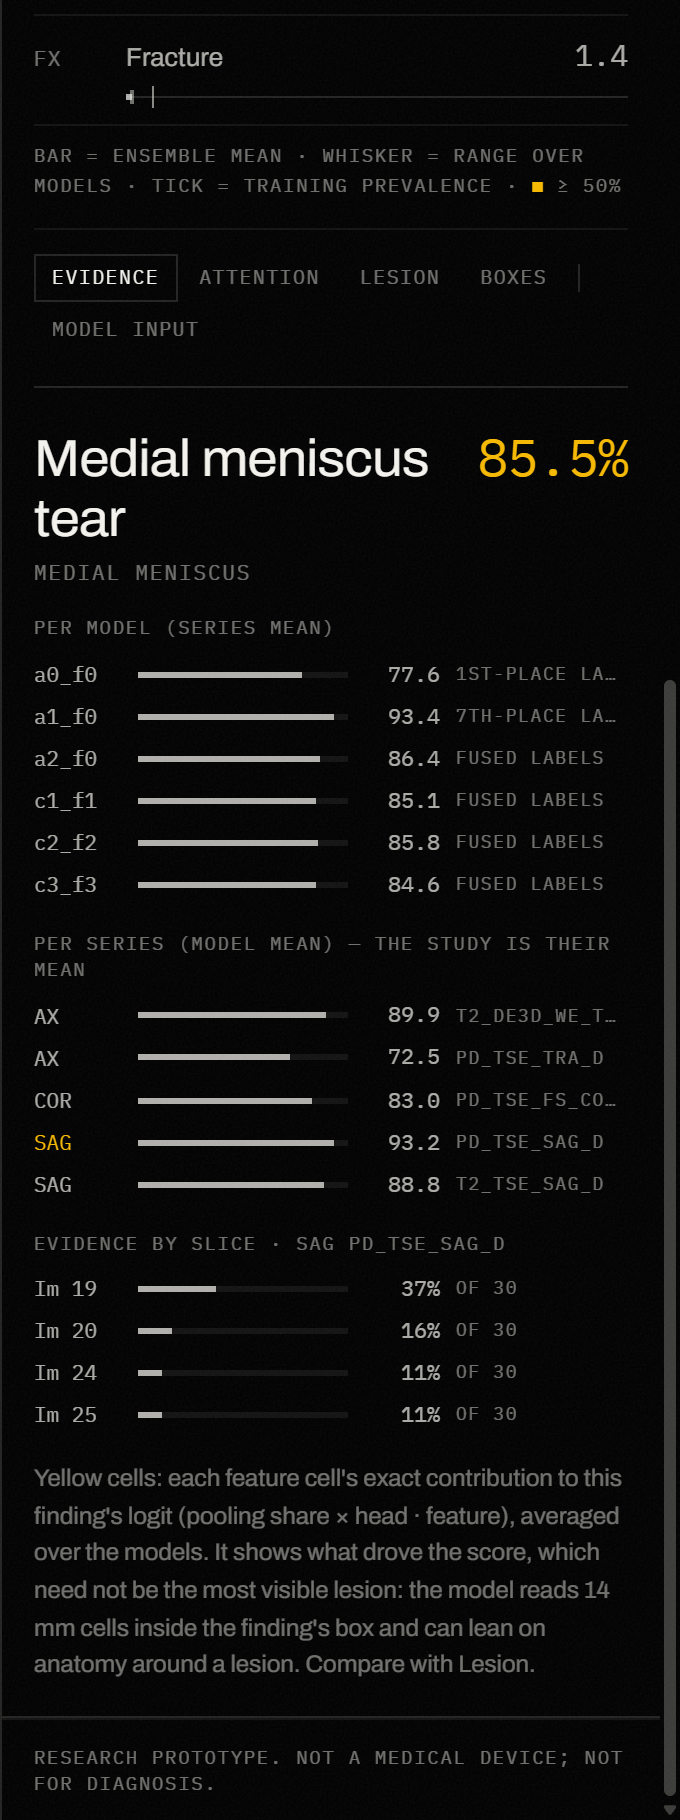
\includegraphics[height=16.5cm]{ws_findings_detail.png}\\[2pt]
{\footnotesize\itshape (b) detail of one finding}
\end{minipage}
\caption[Workstation panels]{Workstation panels: (a) the loaded series with the timed inference steps, peak GPU memory and the attribution check; (b) the per-model and per-series probabilities and the slices that contributed most to the medial meniscus score}
\label{fig:ws-detail}
\end{figure}

The workstation fits on the 6~GB laptop GPU. The weights of all eight networks take 863~MB and load in about 10~s. A typical study uses 1.2~GB of GPU memory at peak, and the largest series we tried, 160 slices of 640 $\times$ 1280 pixels, used 3.1~GB. A typical study takes 4--11~s once the GPU is warm. The study in Figure~\ref{fig:ws-detail} is a heavier case with a 160-slice three-dimensional series: the side classifier took 5.0~s, the detector 3.0~s and the six classifiers 5.6~s, 13.6~s in all, with a peak of 3.3~GB. No quantisation was needed, so the predictions are those of the Kaggle pipeline (Section~\ref{sec:testing}).

During testing, one team member noticed that the evidence for patellofemoral OA peaked on a different slice from the most visible dark lesion. We checked the slice mapping and found it correct, since the model's evidence for that finding really did peak on the patella. This was the reason the lesion overlay and the per-slice breakdown were added, so that a user can compare the two localisations directly.

% ----------------------------------------------------------------------
\section{Testing and Verification}
\label{sec:testing}

Testing in this project covered both the software and the reported results. Table~\ref{tab:tests} lists the main tests and their outcomes.

\begin{table}[htbp]
\centering\footnotesize\setstretch{1}
\caption{Tests and verification checks with their outcomes}
\label{tab:tests}
\begin{tabularx}{\textwidth}{C{0.8cm} L{3.6cm} Y L{2.5cm}}
\toprule
No. & Check & Method & Result \\
\midrule
T1 & Compressed DICOM decoding & training slices converted to JPEG-Lossless and JPEG~2000, decoded and compared & bit-identical \\
T2 & Inference failure handling & six local cases: normal run; damaged fluid-sensitive series; missing plane; missing decoders; mixed ensemble; damaged end and middle slices & fallback, mask, abort, mean, drop and reject as designed \\
T3 & Notebook end to end & each generated notebook run in a fresh interpreter, including the exact upload folder & valid submission files \\
T4 & Float16 on T4 & predictions compared with float32 & max $|\Delta p| = 0.0014$, Spearman $\geq 0.9998$ \\
T5 & Train/test preprocessing parity & same series through both code paths & bit-identical on 51 series \\
T6 & Slice ordering & monotonic positions in a 2,000-series sample & no violations \\
T7 & Single-pass rewrite (Stage 4) & rewritten stage against the separate stage on gold-58 & equal on 57 of 58 studies \\
T8 & Box-pooling inference script & our pipeline against the published notebook, 16 gold studies & correlation 0.996 \\
T9 & Kaggle rehearsal & CPU session, every batch forced to fail once & 15/15 series recovered, 202~s \\
T10 & Reproduction of a published result & model A0 late-submitted & 0.955 private vs 0.954 published \\
T11 & Sharpening switch & $s=1$ against the unmodified model & max difference 0.0 \\
T12 & Workstation fidelity & engine against the Kaggle inference script run locally with the same weights, 3 studies, 90 series--model pairs & max $|\Delta p| = 1.6\times10^{-4}$ \\
T13 & Attribution exactness & sum of cell contributions plus bias against the logit & $5\times10^{-7}$ (fp32), $\leq 0.05$ (fp16) \\
T14 & Sealed gold evaluation & scoring script writes a lock file first and refuses a second run & enforced \\
\bottomrule
\end{tabularx}
\end{table}

\paragraph{Software tests.} Tests T1--T6 were run before the Stage~3 submission. The decoder test (T1) matters because the hidden test set could not be inspected and its run log is not shown to participants, so a silent decoding failure would have been invisible. T4 shows that running in float16 on Kaggle's T4 GPUs changes the probabilities by at most 0.0014 and leaves their order practically unchanged, which is what the AUC depends on. T8--T10 together show that the post-competition inference pipeline reproduces the published model, first on the predictions of the published notebook and then on the private leaderboard. T12 was re-run after every change to the workstation engine; the remaining difference of $1.6\times10^{-4}$ comes from float16 rounding.

\paragraph{Verification of results.} Our own Stage~3 model was never selected on gold-58, and its gold predictions were sealed until the choice was fixed (T14). In Stage~5 no epoch or model was chosen on gold-58. The exceptions were in Stage~4, where public models and blends were compared on gold-58 and the last-day blends were fitted to it. Comparisons between our own models on the same studies are paired and carry bootstrap intervals; leaderboard scores and the single scores of public models do not. Every leaderboard score in Figure~\ref{fig:leaderboard} and Tables~\ref{tab:endgame} and \ref{tab:late} was read from the Kaggle submission history, apart from the three late-submission rows marked as coming from the project log. The figures in this report were drawn by scripts in the report folder from aggregate tables that those scripts compute from the project's run outputs.

\paragraph{Problems found by testing and operation.} Not every problem was caught by a test before it happened. Once, the scripts that polled Kaggle froze for about three hours while the laptop slept, and once two copies of a hand-over script ran at the same time for five hours because stopping the parent process did not stop its child shells; they submitted the same notebook twice. The scripts were rewritten as single processes with a state file and a request to Windows to stay awake. On the last day of the competition, as described in Section~\ref{sec:impl-endgame}, submissions that ran close to the nine-hour limit produced low scores. Both lessons fed into the post-competition work, where run time was budgeted with a margin and every automatic step was made safe to repeat.

\paragraph{Summary of results.} Table~\ref{tab:summary} brings together the main measured results of the project.

\begin{table}[htbp]
\centering\footnotesize\setstretch{1}
\caption{Summary of the main results (macro AUC)}
\label{tab:summary}
\begin{tabular}{L{6.6cm}C{1.9cm}C{1.9cm}C{1.9cm}}
\toprule
System & Gold-58 & Public LB & Private LB \\
\midrule
Frozen EfficientNet-B0, own DICOM pipeline (Stage 1) & 0.753$^{\dagger}$ & 0.775 & 0.755 \\
Fine-tuned 2.5D MIL ensemble F1--F3, report labels (Stage 3) & 0.906 & 0.927 & 0.916 \\
Final competition picks, public models (Stage 4) & -- & 0.958 & 0.943 \\
2.5D MIL, fused image-read labels, one fold (Stage 5) & 0.928 & -- & -- \\
Box-pooling, fused labels, one model A2 (Stage 5) & 0.938 & 0.968 & 0.958 \\
Box-pooling, mean of A0, A1, A2 and C1 (Stage 5) & -- & 0.968 & 0.958 \\
Box-pooling, mean of six models (Stage 5) & 0.941 & not scored & not scored \\
Winning team of the competition & -- & -- & 0.960 \\
\bottomrule
\multicolumn{4}{l}{\scriptsize $^{\dagger}$ the frozen-feature design re-run under the Stage 3 protocol (E0).}
\end{tabular}
\end{table}

% ======================================================================
\chapter[CONCLUSION AND FUTURE SCOPE]{Conclusion and Future Scope}
\label{ch:conclusion}
% ======================================================================

\section{Conclusion}

This project built a deep learning system that reads a complete knee MRI study and estimates the probability of twelve abnormalities, trained on data in which only 58 of 4,407 studies had expert labels. It covered all seven objectives of Section~\ref{sec:objectives}.

Our own pipeline turned multilingual reports into soft labels with a locally run language model (gold agreement 0.868 alone, 0.890 when averaged with two public label sets) and trained a fine-tuned 2.5D multiple-instance network on them. It improved on the frozen-feature design from 0.775 to 0.927 on the public leaderboard (0.755 to 0.916 private). In the final week we built, tested and re-engineered ensembles around the strongest public models, after tracing their training data, and reached 0.958 public and 0.943 private, 490th of 6,299 teams and a bronze medal; the pick that scored 0.943 contains a model trained with an auxiliary task on fastMRI+ data.

The most useful finding came after the competition. By changing only the label file, we showed that our model was limited more by its labels than by its design, since image-read labels raised its gold-58 score from 0.891 to 0.928. Retraining the winning team's published pipeline reproduced its published score, and training it on the mean of two image-read label sets gave 0.958 on the private leaderboard, against 0.960 for the winning team. We also learned to distrust small gains measured on 58 studies. The fastMRI-free blend whose weights were fitted on gold-58 scored 0.935 private, below the 0.940 of the blend it extended.

The local workstation runs all eight networks on a 6~GB laptop GPU, matches our Kaggle inference script to within $1.6\times10^{-4}$, and shows for each model an exact breakdown of its score over image regions. The system remains a research prototype. Its labels are estimates, and it has not been tested on data from other hospitals.

\section{Future Scope}

\begin{itemize}[leftmargin=1.4em]
\item \textbf{Score the pre-registered ensemble.} The six-model ensemble fixed before the last folds were trained has not yet been scored on the private leaderboard. Fixing its notebook and submitting it is the first step.
\item \textbf{Better labels.} Labels were the largest lever in this project. Labels from a vision--language model that reads the images as well as the report could be produced locally and fused with the published sets, and expert semi-quantitative grades such as MOAKS \cite{hunter2011moaks} from the OAI could supervise the osteoarthritis findings directly.
\item \textbf{Teacher--student training.} Out-of-fold predictions of the current models could be mixed with the labels and used to train a new generation of models, in the manner of noisy-student training \cite{xie2020noisystudent}.
\item \textbf{Combining planes.} Both models average evidence across planes. A model that relates the same anatomy in the sagittal, coronal and axial series could help findings such as meniscal tears that are judged on two planes together.
\item \textbf{Weak findings.} Lateral OA and bone contusion remain weaker in the box-pooling ensemble than in our Stage~3 model, and lateral meniscal tears are weak in both; these deserve targeted study.
\item \textbf{External validation.} Testing on studies from hospitals and scanners not seen in training, and reader studies with radiologists, would be required before any clinical use.
\item \textbf{Efficiency.} Compiling the networks with an inference engine and reading DICOM files faster would cut the run time, which matters both for clinical use and for the competition's efficiency track.
\end{itemize}


% ---------------------------------------------------------------- references and appendix
% References in the department's style (IEEE-like). Every entry was checked against Crossref, the publisher,
% the proceedings, arXiv or the source page. The order is the order of first citation in the text
% (scripts/order_references.py rewrites it after a compile).
\cleardoublepage
\phantomsection
\addcontentsline{toc}{chapter}{REFERENCES}
\renewcommand{\bibname}{REFERENCES}
\begingroup
\setlength{\itemsep}{2pt}
\begin{thebibliography}{99}
\sloppy\raggedright

\bibitem{bien2018} N. Bien \textit{et al.}, ``Deep-learning-assisted diagnosis for knee magnetic resonance imaging: Development and retrospective validation of MRNet,'' \textit{PLOS Medicine}, vol. 15, no. 11, Art. no. e1002699, Nov. 2018, doi: 10.1371/journal.pmed.1002699.

\bibitem{kaggle_rsna_knee} P.-H. Chen \textit{et al.} (2026). \textit{RSNA Knee Abnormality Detection} [Online]. Kaggle research code competition. Available: \url{https://www.kaggle.com/competitions/rsna-knee-abnormality-detection} (Accessed: 15 Nov. 2026).

\bibitem{rsna2026announce} Radiological Society of North America. (2026, Aug. 5). \textit{RSNA Launches Knee Abnormality Detection AI Challenge} [Online]. Available: \url{https://www.rsna.org/news/2026/august/ai-challenge-knee-mri} (Accessed: 15 Nov. 2026).

\bibitem{hanley1982} J. A. Hanley and B. J. McNeil, ``The meaning and use of the area under a receiver operating characteristic (ROC) curve,'' \textit{Radiology}, vol. 143, no. 1, pp. 29--36, Apr. 1982, doi: 10.1148/radiology.143.1.7063747.

\bibitem{fawcett2006} T. Fawcett, ``An introduction to ROC analysis,'' \textit{Pattern Recognition Letters}, vol. 27, no. 8, pp. 861--874, Jun. 2006, doi: 10.1016/j.patrec.2005.10.010.

\bibitem{fritz2022review} B. Fritz and J. Fritz, ``Artificial intelligence for MRI diagnosis of joints: A scoping review of the current state-of-the-art of deep learning-based approaches,'' \textit{Skeletal Radiology}, vol. 51, no. 2, pp. 315--329, Feb. 2022, doi: 10.1007/s00256-021-03830-8.

\bibitem{stajduhar2017} I. \v{S}tajduhar, M. Mamula, D. Mileti\'{c}, and G. \"{U}nal, ``Semi-automated detection of anterior cruciate ligament injury from MRI,'' \textit{Computer Methods and Programs in Biomedicine}, vol. 140, pp. 151--164, Mar. 2017, doi: 10.1016/j.cmpb.2016.12.006.

\bibitem{zbontar2018fastmri} J. Zbontar \textit{et al.}, ``fastMRI: An open dataset and benchmarks for accelerated MRI,'' arXiv preprint arXiv:1811.08839, 2018.

\bibitem{zhao2022fastmriplus} R. Zhao \textit{et al.}, ``fastMRI+, Clinical pathology annotations for knee and brain fully sampled magnetic resonance imaging data,'' \textit{Scientific Data}, vol. 9, no. 1, Art. no. 152, Apr. 2022, doi: 10.1038/s41597-022-01255-z.

\bibitem{nevitt_oai} NIMH Data Archive, National Institutes of Health. \textit{The Osteoarthritis Initiative (OAI)} [Online]. Available: \url{https://nda.nih.gov/oai/} (Accessed: 15 Nov. 2026).

\bibitem{ilse2018} M. Ilse, J. M. Tomczak, and M. Welling, ``Attention-based deep multiple instance learning,'' \textit{Proceedings of the 35th International Conference on Machine Learning (ICML)}, Stockholm, Sweden, 2018, PMLR vol. 80, pp. 2127--2136.

\bibitem{deng2009imagenet} J. Deng, W. Dong, R. Socher, L.-J. Li, K. Li, and L. Fei-Fei, ``ImageNet: A large-scale hierarchical image database,'' \textit{IEEE Conference on Computer Vision and Pattern Recognition (CVPR)}, Miami, FL, USA, 2009, pp. 248--255, doi: 10.1109/CVPR.2009.5206848.

\bibitem{tan2019effnet} M. Tan and Q. V. Le, ``EfficientNet: Rethinking model scaling for convolutional neural networks,'' \textit{Proceedings of the 36th International Conference on Machine Learning (ICML)}, Long Beach, CA, USA, 2019, PMLR vol. 97, pp. 6105--6114.

\bibitem{tan2021effnetv2} M. Tan and Q. V. Le, ``EfficientNetV2: Smaller models and faster training,'' \textit{Proceedings of the 38th International Conference on Machine Learning (ICML)}, Virtual Event, 2021, PMLR vol. 139, pp. 10096--10106.

\bibitem{liu2022convnext} Z. Liu, H. Mao, C.-Y. Wu, C. Feichtenhofer, T. Darrell, and S. Xie, ``A ConvNet for the 2020s,'' \textit{IEEE/CVF Conference on Computer Vision and Pattern Recognition (CVPR)}, New Orleans, LA, USA, 2022, pp. 11966--11976, doi: 10.1109/CVPR52688.2022.01167.

\bibitem{dai2021coatnet} Z. Dai, H. Liu, Q. V. Le, and M. Tan, ``CoAtNet: Marrying convolution and attention for all data sizes,'' \textit{Advances in Neural Information Processing Systems 34 (NeurIPS 2021)}, Virtual Event, 2021, pp. 3965--3977.

\bibitem{oquab2024dinov2} M. Oquab \textit{et al.}, ``DINOv2: Learning robust visual features without supervision,'' \textit{Transactions on Machine Learning Research}, Jan. 2024. [Online]. Available: \url{https://openreview.net/forum?id=a68SUt6zFt}

\bibitem{irvin2019chexpert} J. Irvin \textit{et al.}, ``CheXpert: A large chest radiograph dataset with uncertainty labels and expert comparison,'' \textit{Proceedings of the AAAI Conference on Artificial Intelligence}, Honolulu, HI, USA, 2019, vol. 33, no. 1, pp. 590--597, doi: 10.1609/aaai.v33i01.3301590.

\bibitem{smit2020chexbert} A. Smit, S. Jain, P. Rajpurkar, A. Pareek, A. Y. Ng, and M. P. Lungren, ``Combining automatic labelers and expert annotations for accurate radiology report labeling using BERT,'' \textit{Proceedings of the 2020 Conference on Empirical Methods in Natural Language Processing (EMNLP)}, Online, 2020, pp. 1500--1519, doi: 10.18653/v1/2020.emnlp-main.117.

\bibitem{jain2021visualchexbert} S. Jain \textit{et al.}, ``VisualCheXbert: Addressing the discrepancy between radiology report labels and image labels,'' \textit{Proceedings of the ACM Conference on Health, Inference, and Learning (CHIL '21)}, Virtual Event, USA, 2021, pp. 105--115, doi: 10.1145/3450439.3451862.

\bibitem{qwen2025qwen25} Qwen Team (A. Yang \textit{et al.}), ``Qwen2.5 technical report,'' arXiv preprint arXiv:2412.15115, 2024.

\bibitem{yang2025qwen3} A. Yang \textit{et al.}, ``Qwen3 technical report,'' arXiv preprint arXiv:2505.09388, 2025.

\bibitem{tascj_boxpool} tascj (tascj0). (2026). \textit{RSNA 2026 Knee Box-Pooling Classifier} [Online]. Kaggle notebook, Apache 2.0 licence. Available: \url{https://www.kaggle.com/code/tascj0/rsna-2026-knee-box-pooling-classifier} (Accessed: 15 Nov. 2026).

\bibitem{songqizhou_llmlabels} BarryZhou (songqizhou). (2026, Oct. 24). \textit{RSNA Knee LLM Labels} [Online]. Kaggle dataset, CC BY-NC-SA 4.0 licence. Available: \url{https://www.kaggle.com/datasets/songqizhou/rsna-knee-llm-labels} (Accessed: 15 Nov. 2026).

\bibitem{efron1993} B. Efron and R. J. Tibshirani, \textit{An Introduction to the Bootstrap}. New York, NY, USA: Chapman \& Hall, 1993.

\bibitem{wightman2019timm} R. Wightman. (2019). \textit{PyTorch Image Models} [Online]. GitHub repository, doi: 10.5281/zenodo.4414861. Available: \url{https://github.com/huggingface/pytorch-image-models} (Accessed: 15 Nov. 2026).

\bibitem{loshchilov2019adamw} I. Loshchilov and F. Hutter, ``Decoupled weight decay regularization,'' \textit{International Conference on Learning Representations (ICLR)}, New Orleans, LA, USA, 2019. [Online]. Available: \url{https://openreview.net/forum?id=Bkg6RiCqY7}

\bibitem{loshchilov2017sgdr} I. Loshchilov and F. Hutter, ``SGDR: Stochastic gradient descent with warm restarts,'' \textit{International Conference on Learning Representations (ICLR)}, Toulon, France, 2017. [Online]. Available: \url{https://openreview.net/forum?id=Skq89Scxx}

\bibitem{tascj_roidetector} tascj (tascj0). (2026). \textit{RSNA 2026 Knee ROI Detector} [Online]. Kaggle notebook, Apache 2.0 licence. Available: \url{https://www.kaggle.com/code/tascj0/rsna-2026-knee-roi-detector} (Accessed: 15 Nov. 2026).

\bibitem{tascj_sideclassifier} tascj (tascj0). (2026). \textit{RSNA 2026 Knee Side Classifier} [Online]. Kaggle notebook, Apache 2.0 licence. Available: \url{https://www.kaggle.com/code/tascj0/rsna-2026-knee-side-classifier} (Accessed: 15 Nov. 2026).

\bibitem{he2016resnet} K. He, X. Zhang, S. Ren, and J. Sun, ``Deep residual learning for image recognition,'' \textit{IEEE Conference on Computer Vision and Pattern Recognition (CVPR)}, Las Vegas, NV, USA, 2016, pp. 770--778, doi: 10.1109/CVPR.2016.90.

\bibitem{he2019bagoftricks} T. He, Z. Zhang, H. Zhang, Z. Zhang, J. Xie, and M. Li, ``Bag of tricks for image classification with convolutional neural networks,'' \textit{IEEE/CVF Conference on Computer Vision and Pattern Recognition (CVPR)}, Long Beach, CA, USA, 2019, pp. 558--567, doi: 10.1109/CVPR.2019.00065.

\bibitem{lin2017fpn} T.-Y. Lin, P. Doll\'{a}r, R. Girshick, K. He, B. Hariharan, and S. Belongie, ``Feature pyramid networks for object detection,'' \textit{IEEE Conference on Computer Vision and Pattern Recognition (CVPR)}, Honolulu, HI, USA, 2017, pp. 936--944, doi: 10.1109/CVPR.2017.106.

\bibitem{perez2018film} E. Perez, F. Strub, H. de Vries, V. Dumoulin, and A. Courville, ``FiLM: Visual reasoning with a general conditioning layer,'' \textit{Proceedings of the AAAI Conference on Artificial Intelligence}, New Orleans, LA, USA, 2018, vol. 32, no. 1, pp. 3942--3951, doi: 10.1609/aaai.v32i1.11671.

\bibitem{tascj_agentlabels} tascj (tascj0). (2026, Oct. 24). \textit{RSNA 2026 Knee agent-made labels} [Online]. Kaggle dataset, CC BY 4.0 licence. Available: \url{https://www.kaggle.com/datasets/tascj0/rsna-2026-knee-agent-labels} (Accessed: 15 Nov. 2026).

\bibitem{fastapi} S. Ram\'{\i}rez. \textit{FastAPI} [Online]. Available: \url{https://fastapi.tiangolo.com} (Accessed: 15 Nov. 2026).

\bibitem{react} Meta Platforms, Inc. \textit{React} [Online]. Available: \url{https://react.dev} (Accessed: 15 Nov. 2026).

\bibitem{vite} VoidZero Inc. and Vite contributors. \textit{Vite} [Online]. Available: \url{https://vite.dev} (Accessed: 15 Nov. 2026).

\bibitem{threejs} three.js authors. \textit{Three.js -- JavaScript 3D Library} [Online]. Available: \url{https://threejs.org} (Accessed: 15 Nov. 2026).

\bibitem{selvaraju2017gradcam} R. R. Selvaraju, M. Cogswell, A. Das, R. Vedantam, D. Parikh, and D. Batra, ``Grad-CAM: Visual explanations from deep networks via gradient-based localization,'' \textit{IEEE International Conference on Computer Vision (ICCV)}, Venice, Italy, 2017, pp. 618--626, doi: 10.1109/ICCV.2017.74.

\bibitem{paszke2019pytorch} A. Paszke \textit{et al.}, ``PyTorch: An imperative style, high-performance deep learning library,'' \textit{Advances in Neural Information Processing Systems 32 (NeurIPS 2019)}, Vancouver, BC, Canada, 2019. [Online]. Available: \url{https://proceedings.neurips.cc/paper/2019/hash/bdbca288fee7f92f2bfa9f7012727740-Abstract.html}

\bibitem{mason_pydicom} D. Mason \textit{et al.} (2026, Mar. 19). \textit{pydicom/pydicom: Pydicom v3.0.2} [Online]. Zenodo, doi: 10.5281/zenodo.19119715. Available: \url{https://github.com/pydicom/pydicom} (Accessed: 15 Nov. 2026).

\bibitem{wolf2020transformers} T. Wolf \textit{et al.}, ``Transformers: State-of-the-art natural language processing,'' \textit{Proceedings of the 2020 Conference on Empirical Methods in Natural Language Processing: System Demonstrations}, Online, 2020, pp. 38--45, doi: 10.18653/v1/2020.emnlp-demos.6.

\bibitem{bitsandbytes} bitsandbytes collective. \textit{bitsandbytes: Accessible large language models via k-bit quantization for PyTorch} [Online]. Available: \url{https://github.com/bitsandbytes-foundation/bitsandbytes} (Accessed: 15 Nov. 2026).

\bibitem{kaggle_cli} Kaggle. \textit{Kaggle CLI: Official Kaggle command-line interface} [Online]. Available: \url{https://github.com/Kaggle/kaggle-cli} (Accessed: 15 Nov. 2026).

\bibitem{micikevicius2018amp} P. Micikevicius \textit{et al.}, ``Mixed precision training,'' \textit{International Conference on Learning Representations (ICLR)}, Vancouver, BC, Canada, 2018. [Online]. Available: \url{https://openreview.net/forum?id=r1gs9JgRZ}

\bibitem{dicom_standard} \textit{Digital Imaging and Communications in Medicine (DICOM) Standard}, NEMA PS3 / ISO 12052, edition 2026d. Rosslyn, VA, USA: National Electrical Manufacturers Association. [Online]. Available: \url{https://www.dicomstandard.org/current} (Accessed: 15 Nov. 2026).

\bibitem{dettmers2023qlora} T. Dettmers, A. Pagnoni, A. Holtzman, and L. Zettlemoyer, ``QLoRA: Efficient finetuning of quantized LLMs,'' \textit{Advances in Neural Information Processing Systems 36 (NeurIPS 2023)}, New Orleans, LA, USA, 2023, pp. 10088--10115, doi: 10.52202/075280-0441.

\bibitem{kwon2023vllm} W. Kwon \textit{et al.}, ``Efficient memory management for large language model serving with PagedAttention,'' \textit{Proceedings of the 29th Symposium on Operating Systems Principles (SOSP '23)}, Koblenz, Germany, 2023, pp. 611--626, doi: 10.1145/3600006.3613165.

\bibitem{dawid1979} A. P. Dawid and A. M. Skene, ``Maximum likelihood estimation of observer error-rates using the EM algorithm,'' \textit{Journal of the Royal Statistical Society. Series C (Applied Statistics)}, vol. 28, no. 1, pp. 20--28, 1979, doi: 10.2307/2346806.

\bibitem{northcutt2021cl} C. Northcutt, L. Jiang, and I. Chuang, ``Confident learning: Estimating uncertainty in dataset labels,'' \textit{Journal of Artificial Intelligence Research}, vol. 70, pp. 1373--1411, Apr. 2021, doi: 10.1613/jair.1.12125.

\bibitem{nartaa_swa} D. Zakaria (nartaa). (2026, Oct. 7). \textit{RSNA Knee selected SWA weights 0949 and 0945} [Online]. Kaggle dataset. Available: \url{https://www.kaggle.com/datasets/nartaa/rsna-knee-publication-swa-weights-20261007} (Accessed: 15 Nov. 2026).

\bibitem{heliosli_compact} Heliosli (heliosli). (2026, Oct. 10). \textit{RSNA Knee Compact v1} [Online]. Kaggle dataset, version 13. Available: \url{https://www.kaggle.com/datasets/heliosli/rsna-knee-compact-v1} (Accessed: 15 Nov. 2026).

\bibitem{nartaa_s6fall} D. Zakaria (nartaa). (2026, Oct. 17). \textit{RSNA Knee S6 ConvNeXt all-data weights 0950} [Online]. Kaggle dataset, version 5. Available: \url{https://www.kaggle.com/datasets/nartaa/rsna-knee-s6fall-weights} (Accessed: 15 Nov. 2026).

\bibitem{rostigor_r6} Igor V (rostigor). (2026, Oct. 15). \textit{RSNA Knee R6 fe055406 versioned} [Online]. Kaggle dataset. Available: \url{https://www.kaggle.com/datasets/rostigor/rsna-knee-r6-fe055406} (Accessed: 15 Nov. 2026).

\bibitem{heliosli_blendgold} Heliosli (heliosli). (2026). \textit{rsna-knee-blend-gold (Dataset restored)} [Online]. Kaggle notebook, Apache 2.0 licence. Available: \url{https://www.kaggle.com/code/heliosli/rsna-knee-blend-gold-dataset-restored} (Accessed: 15 Nov. 2026).

\bibitem{goodpjw_coatnet_nb} goodpjw2008. (2026). \textit{RSNA Knee \textbar{} CoAtNet + R6 + 2.5D MIL \textbar{} LB 0.958} [Online]. Kaggle notebook, Apache 2.0 licence. Available: \url{https://www.kaggle.com/code/goodpjw2008/rsna-knee-coatnet-r6-2-5d-mil-lb-0-958} (Accessed: 15 Nov. 2026).

\bibitem{desai2021skmtea} A. D. Desai \textit{et al.}, ``SKM-TEA: A dataset for accelerated MRI reconstruction with dense image labels for quantitative clinical evaluation,'' \textit{Proceedings of the Neural Information Processing Systems Track on Datasets and Benchmarks}, Virtual Event, 2021, vol. 1. [Online]. Available: \url{https://datasets-benchmarks-proceedings.neurips.cc/paper_files/paper/2021/hash/03c6b06952c750899bb03d998e631860-Abstract-round2.html}

\bibitem{hunter2011moaks} D. J. Hunter \textit{et al.}, ``Evolution of semi-quantitative whole joint assessment of knee OA: MOAKS (MRI Osteoarthritis Knee Score),'' \textit{Osteoarthritis and Cartilage}, vol. 19, no. 8, pp. 990--1002, Aug. 2011, doi: 10.1016/j.joca.2011.05.004.

\bibitem{xie2020noisystudent} Q. Xie, M.-T. Luong, E. Hovy, and Q. V. Le, ``Self-training with noisy student improves ImageNet classification,'' \textit{IEEE/CVF Conference on Computer Vision and Pattern Recognition (CVPR)}, Seattle, WA, USA, 2020, pp. 10684--10695, doi: 10.1109/CVPR42600.2020.01070.

\end{thebibliography}
\endgroup

% ======================================================================
% APPENDIX
% ======================================================================
\cleardoublepage
\phantomsection
\addcontentsline{toc}{chapter}{APPENDIX}
\chapter*{APPENDIX}
\setcounter{section}{0}
\renewcommand{\thesection}{\Alph{section}}
\counterwithin*{table}{section}
\renewcommand{\theHsection}{app.\Alph{section}}
\renewcommand{\theHtable}{app.\Alph{section}.\arabic{table}}
\renewcommand{\thetable}{\Alph{section}.\arabic{table}}
\setcounter{table}{0}

\section{Project Team and Supervision}

\begin{table}[H]
\centering\footnotesize\setstretch{1}
\caption{Project team (all students of B.Tech Electronics \& Communication Engineering, Section B)}
\label{tab:team}
\begin{tabular}{L{4.2cm}L{3.0cm}L{6.2cm}}
\toprule
Name & University roll no. & E-mail \\
\midrule
Nishkarsh Singhal & 24294917099 & Nishkarsh.5108@ece.du.ac.in \\
Anuj Chaubey & 24294917055 & anujchaubey3669@ece.du.ac.in \\
Vardhan Harsh Nigam & 24294917014 & Vardhanharshnigam@ece.du.ac.in \\
\bottomrule
\end{tabular}
\end{table}

The project was supervised by Dr.\ Varun Saxena, Associate Professor, Department of Electronics \& Communication Engineering (varunsaxena@ece.du.ac.in), with Dr.\ Sangeeta Yadav, Assistant Professor, Department of Computer Science \& Engineering (Sangeeta@fot.du.ac.in), as co-supervisor.

\section{Complete Submission History}

Table~\ref{tab:allsubs} lists every submission made from the team's Kaggle account, read from the Kaggle submission history through the command-line client. The reference number is Kaggle's own identifier. Scores are macro AUC on the public and private leaderboards. Submissions~1--16 were made during the competition and 17--22 after it closed.

\begin{longtable}{C{0.6cm}C{1.5cm}L{2.2cm}L{6.9cm}C{1.1cm}C{1.1cm}}
\caption{All submissions from the team's account, in the order made}\label{tab:allsubs}\\
\toprule
No. & Reference & Stage & Content & Public & Private \\
\midrule
\endfirsthead
\toprule
No. & Reference & Stage & Content & Public & Private \\
\midrule
\endhead
1 & 55906095 & Stage 1 & v1: frozen EfficientNet-B0 on a third-party cache & 0.500 & 0.498 \\
2 & 55966953 & Stage 1 & v2: frozen EfficientNet-B0 on our own DICOM pipeline & 0.775 & 0.755 \\
3 & 57336780 & Stage 3 & 2.5D MIL ConvNeXt-T, 3 seeds (F1--F3), shift TTA & 0.927 & 0.916 \\
4 & 57365203 & Stage 3 & F1--F3 + high-resolution model E9 & 0.928 & 0.915 \\
5 & 57384567 & Stage 4 & A-strict: public CoAtNet (OAI) + public S6 & 0.954 & 0.937 \\
6 & 57384570 & Stage 4 & A-strict+: public 0.958 notebook with R6 replaced by S6 & 0.954 & 0.937 \\
7 & 57406523 & Stage 4 & final-strict: A-strict + public s6fall (fastMRI-free) & 0.956 & 0.940 \\
8 & 57444580 & Stage 4 & final-max v1: public CoAtNet + R6 notebook + s6fall & 0.958 & 0.943 \\
9 & 57460890 & Stage 4 & final-max v2: s6fall scored inside the R6 pass & 0.958 & 0.943 \\
10 & 57480525 & Stage 4 & final-max v3: + our fine-tuned s6ft\_v2, s6ft\_v1 & 0.958 & 0.943 \\
11 & 57480912 & Stage 4 & final-strict-v2: + our fine-tunes & 0.956 & 0.940 \\
12 & 57512015 & Stage 4 (last day) & final-max v4: specialist routing (no score returned) & -- & -- \\
13 & 57519582 & Stage 4 (last day) & final-strict-v3: specialist routing fitted on gold-58 & 0.948 & 0.935 \\
14 & 57521956 & Stage 4 (last day) & final-max (kernel v8): stopped by its 8.3 h deadline & 0.891 & 0.894 \\
15 & 57531417 & Stage 4 (last day) & final-max (kernel v9): same blend, later version & 0.848 & 0.850 \\
16 & 57534028 & Stage 4 (last day) & final-max (kernel v10): stride-2 master blend & 0.866 & 0.870 \\
17 & 58350230 & Stage 5 & box-pooling, fused labels, fold 0 (A2) & 0.968 & 0.958 \\
18 & 58350257 & Stage 5 & box-pooling, fused labels, folds 0+1 (A2 + C1) & 0.968 & 0.958 \\
19 & 58369148 & Stage 5 & A1 with per-finding attention sharpening & 0.967 & 0.957 \\
20 & 58369192 & Stage 5 & mean of A0, A1, A2 & 0.968 & 0.958 \\
21 & 58369222 & Stage 5 & A1 with attention sharpening s = 2 & 0.967 & 0.956 \\
22 & 58369269 & Stage 5 & mean of A0, A1, A2, C1 & 0.968 & 0.958 \\
\bottomrule
\end{longtable}

\section{Training Recipe of the Box-Pooling Models}

\begin{table}[H]
\centering\footnotesize\setstretch{1}
\caption[Training settings of the box-pooling models]{Settings used for the six box-pooling training runs of Stage 5 (published recipe; labels, folds and switches set by our notebook builder)}
\label{tab:bprecipe}
\begin{tabularx}{\textwidth}{L{4.0cm} Y}
\toprule
Item & Setting \\
\midrule
Encoder & ConvNeXt-Tiny (ImageNet-12k pretrained, ImageNet-1k fine-tuned), drop-path 0.1; 31.0~M parameters with all heads \\
Input & every slice resampled to a 140~mm field at 384 pixels (0.365~mm per pixel); 112~mm crop at 256 pixels; at most 64 slices per series; intensity window at the 0.5 and 99.5 percentiles \\
Pooling & 8 $\times$ 8 feature cells per slice; per-finding three-dimensional box from the detector; in-box attention initialised to zero \\
Loss & binary cross-entropy + 1.0 $\times$ lesion-coverage loss + 0.3 $\times$ report-embedding loss (Equation~\ref{eq:bploss}) \\
Labels & first-place, seventh-place or fused image-read labels; gold studies never trained on \\
Optimiser & AdamW, learning rate $5\times10^{-5}$, weight decay 0.02, 0.5 epoch warm-up, gradient clipping at 1.0 \\
Batch & 8 series per update, as 2 series per micro-batch on each of 2 GPUs with gradient accumulation \\
Precision and EMA & float16 with gradient scaling; EMA decay 0.999; the EMA weights are evaluated and used \\
Augmentation & scale 0.9--1.1, shift $\pm8\%$, rotation $\pm10^\circ$ \\
Folds & the published 5-fold split of the 4,349 non-gold studies (seed 42); runs on folds 0--3 with seed 3; 8 epochs \\
\bottomrule
\end{tabularx}
\end{table}

\section{Organisation of the Source Code}

\begin{table}[H]
\centering\footnotesize\setstretch{1}
\caption{Main source folders and scripts of the project}
\label{tab:code}
\begin{tabularx}{\textwidth}{L{5.0cm} Y}
\toprule
Location & Purpose \\
\midrule
\texttt{src/model/}, \texttt{src/label\_generation/} & Stage 1: first labeller, consensus aggregation and frozen-feature models \\
\texttt{src/audit/} & Stage 2: DICOM header inventory, EDA, laterality table, decoder self-test \\
\texttt{src/labeling/} & Stage 2: forced-choice LLM labeller, rule extractor, label validation and downstream test \\
\texttt{src/imaging/} & Stage 3: study index, decoding, data loader, 2.5D model, training, prediction, run queue and tests \\
\texttt{notebooks/} & generated Kaggle notebooks for training, inference and the competition endgame, with their builders and local tests \\
\texttt{src/emergency/} & Stage 4: local runs of public models on gold-58, blend evaluation, single-pass rewrite and fine-tuning \\
\texttt{src/postcomp/} & Stage 5: training and inference notebook builders, inference script, scoring, sharpening sweep, series weighting and hand-over scripts \\
\texttt{demo/server/}, \texttt{demo/web/} & Stage 6: workstation server, engine, fidelity test and browser application \\
\texttt{reports/SEC project report/} & this report: \LaTeX\ source, figures, aggregate data tables and the scripts that produce them \\
\bottomrule
\end{tabularx}
\end{table}

\section{Reproducing the Figures of this Report}

The data figures were produced in three steps by scripts kept in the \texttt{scripts} folder of this report. \texttt{collect\_results.py} reads the project's run outputs and writes only aggregate tables (counts, rates, AUCs and confidence intervals) to the \texttt{data} folder; it writes no per-study rows, report text or images. \texttt{prepare\_submissions.py} converts the Kaggle submission export into the table of Appendix~B without dates. \texttt{make\_figures.py} draws Figures~\ref{fig:dataset}, \ref{fig:labels}, \ref{fig:curves}, \ref{fig:ablation}, \ref{fig:attention}, \ref{fig:gold}, \ref{fig:leaderboard}, \ref{fig:labelswap} and \ref{fig:sharpen} from those tables. The workstation screenshots were captured by \texttt{capture\_workstation.mjs} through a headless browser and cut into the report's panels by \texttt{prepare\_screenshots.py}. All bootstrap intervals use 2,000 resamples of studies, except the sharpening sweep, which uses 1,000.


\end{document}
